%%
%% This is file `02_article1.tex',
%% generated with the docstrip utility.
%%
%% The original source files were:
%%
%% dms.dtx  (with options: `article')
 
%% To change chapter header dynamically from french to english, use
\entetedynamique
\setcounter{corA}{0} % Pour recommancer à compter les def,
                     % theo, etc. à partir de 1
 % Pour écrire un article en français
%% \francais
 % Pour écrire un article en anglais
\anglais
%% NOTE: La plupart des macros ont un nom en anglais.
%% P.ex. \adresse et \address fonctionnent et sont équivalents.
%% \revue=\journal
%% \auteur=\author
%% \titre=\title

%% Les contributions apparaîtront habituellement après
%% \maketitle (voir un peu plus bas). Selon les goûts, il est
%% possible de mettre les contributions
%% avant la page titre de l'article, simplement en les écrivant
%% directement ici. Par exemple :
 % \cleardoublepage
 % \pdfbookmark[chapter]{Contributions}{contrib1} % Remplacer par contrib2 pour l'article 2 etc.
 % {\bfseries\Large\noindent Contributions de <mon nom> et rôle joué par les coauteurs}
 % J'ai contribué en...
 %
 % Le rôle des coauteurs a été de...

%% Nom de la revue de publication
\revue{EcoEvoRxiv and can be found at https://doi.org/10.32942/X28G8Z}
\article{Deciphering probabilistic species interaction networks}\label{chapter1}
%% On peut se référer aux numéros de chapitre ou d'article comme suit.
%% Si on fait
%% \label{chap:article1},
%% alors \ref{chap:article1} donnera le numéro du chapitre. On peut ensuite faire
%% \labelart{art:article1}
%% et alors \ref{art:article1} donnera le numéro d'article.
%% Par exemple, si cette article est le premier article et le deuxième chapitre,
%% alors si on écrit
%% Voir le chapitre~\ref{chap:article1} (l'article~\ref{art:article1}).
%% deviendra
%% Voir le chapitre 2 (l'article 1).
%% Si on veut écrire « premier article » au lieu « article 1 », on peut
%% simplement faire
%% \ordinal{\ref{art:article1}}~article  % devient première article
%% ou
%% \Ordinal{\ref{art:article1}}~article  % devient Première article (avec la majuscule)
%% Si on est en mode \anglais, \ordinal écrire first, second,...

 % Contribution(s) peronnelle(s) à l'article et rôle joué par tous les coauteur·e·s
 %
 % Nécessaire seulement lorsque vous n'êtes pas seul·e auteur·e.
 % Les contributions peuvent apparaître ailleur dans la thèse.
 % Si \contributions est laissé vide (p.ex. si vous effacez
 % celui ci-bas), aucune contributions ne seront générées sur
 % la page titre de l'article. Vous pouvez alors mettre un
 % \newpage si vous souhaitez que les résumé et abstract soient
 % la page suivante.
 %
 % REMARQUE : À peu près toutes les constructions \LaTeX\ sont permises
 % dans les contributions.
 %
 % La commande admet une option [<entête>]
\contributions%[Mes contributions et le rôle des coauteurs]
{

FB developed and performed the analyses and wrote the first and final versions
of the manuscript. All authors participated in the conceptualisation and
revision of the manuscript. DG and TP provided guidance on the analyses and
interpretation of the results. All authors read and approved the
manuscript.\\[1cm]

  % Exemple avec un <itemize>
  %  \begin{itemize}
  %      \item Calcul de telle chose;
  %      \item Vérification de telle équation;
  %      \item Idée pour telle définition;
  %      \item Démonstration de tel théorème.
  %  \end{itemize}
}

%%% INFORMATIONS POUR LA PAGE TITRE
 % Premier auteur·e et adresse
\auteur{Francis Banville}
\adresse{Département de sciences biologiques, Université de Montréal
\\1375 avenue Thérèse-Lavoie-Roux, Montréal, QC, Canada H2V 0B3}

% Deuxième auteur·e et adresse (si différente de la première)
\auteur{Tanya Strydom}
\adresse{Département de sciences biologiques, Université de Montréal
\\1375 avenue Thérèse-Lavoie-Roux, Montréal, QC, Canada H2V 0B3}
 
%% et ainsi de suite pour les autres auteurs
\auteur{Penelope S.A. Blyth}
\adresse{School of Biosciences, The University of Sheffield
\\Western Bank, Sheffield, United Kingdom S10 2TN}
 
\auteur{Chris Brimacombe}
\adresse{Department of Ecology and Evolutionary Biology, University of Toronto
\\25 Willcocks St, Toronto, ON, Canada M5S 3B2}

\auteur{Michael D. Catchen}
\adresse{Department of Biology, McGill University 
\\1205 avenue du Docteur-Penfield, Montréal, QC, Canada H3A 1B1}

\auteur{Gabriel Dansereau}
\adresse{Département de sciences biologiques, Université de Montréal
\\1375 avenue Thérèse-Lavoie-Roux, Montréal, QC, Canada H2V 0B3}
 
\auteur{Gracielle Higino}
\adresse{Département de biologie, Université de Sherbrooke
\\2500 boulevard de l'Université, Sherbrooke, Qc, Canada J1K 2R1}
 
\auteur{Thomas Malpas}
\adresse{School of Biosciences, The University of Sheffield
\\Western Bank, Sheffield, United Kingdom S10 2TN}
 
\auteur{Hana Mayall}
\adresse{School of Biosciences, The University of Sheffield
\\Western Bank, Sheffield, United Kingdom S10 2TN}
 
\auteur{Kari Norman}
\adresse{Département de sciences biologiques, Université de Montréal
\\1375 avenue Thérèse-Lavoie-Roux, Montréal, QC, Canada H2V 0B3}
 
\auteur{Dominique Gravel}
\adresse{Département de biologie, Université de Sherbrooke
\\2500 boulevard de l'Université, Sherbrooke, Qc, Canada J1K 2R1}
 
\auteur{Timothée Poisot}
\adresse{Département de sciences biologiques, Université de Montréal
\\1375 avenue Thérèse-Lavoie-Roux, Montréal, QC, Canada H2V 0B3}
 
\maketitle

\begin{resume}{réseaux écologiques, réseaux trophiques, metaweb, réseaux probabilistes, échelle spatiale, interactions entre espèces, échelle temporelle}
  Représenter les interactions entre espèces de manière probabiliste (quelle est
  leur probabilité d'occurrence?) plutôt que de manière déterministe (se
  produisent-elles?) nous informe de leur variabilité et des incertitudes dans
  nos connaissances des interactions. Les sources d'incertitude capturées par
  les probabilités d'interaction dépendent de la méthode utilisée pour les
  évaluer : incertitude des modèles prédictifs, évaluation subjective des
  experts ou mesure empirique de la variabilité spatio-temporelle des
  interactions. Cependant, des directives pour l'estimation et la documentation
  des données d'interactions probabilistes sont manquantes. Cela est préoccupant
  car notre compréhension et l'analyse des probabilités d'interaction dépendent
  de leur définition parfois ambiguë et de leurs sources d'incertitude. Nous
  passons en revue comment les interactions probabilistes sont définies à
  différentes échelles spatiales, des interactions locales aux réseaux régionaux
  (\textit{metawebs}), en mettant l'accent sur les interactions hôte-parasites
  et trophiques (prédation et herbivorie). Ces définitions reposent sur la
  distinction entre la réalisation d'une interaction à un moment et un lieu
  spécifiques (local) et sa faisabilité biologique ou écologique (régional). En
  utilisant des données d'interactions hôtes-parasites en Europe, nous
  illustrons comment ces deux représentations de réseau diffèrent dans leurs
  propriétés statistiques, en particulier : comment les réseaux locaux et les
  \textit{metawebs} diffèrent dans leurs mises à l'échelle spatiale et
  temporelle des probabilités d'interaction, mais pas dans leur mise à l'échelle
  taxonomique. Nous présentons deux approches pour inférer des interactions
  binaires à partir d'interactions probabilistes qui tiennent compte de ces
  différences et montrons que des biais systématiques apparaissent lorsque l'on
  infère directement des réseaux locaux à partir d'un \textit{metaweb}. Nos
  résultats soulignent l'importance de descriptions plus rigoureuses des réseaux
  d'interactions probabilistes entre espèces qui spécifient leur type
  d'interaction (locale ou régionale), leurs variables conditionnelles et leurs
  sources d'incertitude.
\end{resume}

\begin{abstract}{ecological networks, food webs, metaweb, probabilistic networks, spatial scale, species interactions, temporal scale}
  Representing species interactions probabilistically (how likely are they to
  occur?) as opposed to deterministically (are they occurring?) conveys
  uncertainties in our knowledge of interactions and information on their
  variability. The sources of uncertainty captured by interaction probabilities
  depend on the method used to evaluate them: uncertainty of predictive models,
  subjective assessment of experts, or empirical measurement of interaction
  spatiotemporal variability. However, guidelines for the estimation and
  documentation of probabilistic interaction data are lacking. This is
  concerning because our understanding and analysis of interaction probabilities
  depend on their sometimes elusive definition and uncertainty sources. We
  review how probabilistic interactions are defined at different spatial scales,
  from local interactions to regional networks (metawebs), with a strong
  emphasis on host-parasite and trophic (predatory and herbivory) interactions.
  These definitions are based on the distinction between the realization of an
  interaction at a specific time and space (local) and its biological or
  ecological feasibility (regional). Using host-parasite interactions in Europe,
  we illustrate how these two network representations differ in their
  statistical properties, specifically: how local networks and metawebs differ
  in their spatial and temporal scaling of probabilistic interactions, but not
  in their taxonomic scaling. We present two approaches to inferring binary
  interactions from probabilistic ones that account for these differences and
  show that systematic biases arise when directly inferring local networks from
  metawebs. Our results underscore the importance of more rigorous descriptions
  of probabilistic species interaction networks that specify their type of
  interaction (local or regional), conditional variables and uncertainty
  sources.  
\end{abstract}

\clearpage

\section{Introduction}
%%
% Exemple de citation~: Consultez le \LaTeX\ companien
% de Mittelbach {\it et al\/}~\cite{exemple}.

%Imports bibliography file

\subsection{Species interactions are variable and uncertain}

As we try to navigate global biodiversity change, filling in knowledge gaps
about biodiversity becomes instrumental to monitoring and mitigating those
changes (\cite{Hortal2015Seven}, \cite{Gonzalez2022Monitor},
\cite{Abrego2021Accounting}). However, cataloging species, populations and, in
particular, ecological interactions (e.g., predation, parasitism, and
pollination) is a substantial challenge (\cite{Polis1991Complex},
\cite{Pascual2006Ecological}). There are methodological and biological
constraints that hinder our ability to document species interactions, inevitably
leading to uncertainty in our knowledge of interactions. For example, the
spatial and temporal uncoupling of species (e.g., nocturnal and diurnal species
coexisting in the same space with different daily activity timings,
\cite{Jordano1987Patterns}) and the large number of rare and cryptic
interactions in a community, contribute to these knowledge gaps by making it
more difficult to observe interactions (\cite{Jordano2016Sampling}). 

Several conditions must be satisfied for an interaction to be observed locally.
First, both species must have overlapping geographic ranges, i.e. they must
co-occur within the region of interest (\cite{Morales-Castilla2015Inferring},
\cite{Cazelles2016Theorya}). Second, they must have some probability of meeting
within a defined time frame (\cite{Poisot2015Species}). Probabilities of
interspecific encounters are typically low, especially for rare species with low
abundances (\cite{Vazquez2007Species}, \cite{Canard2012Emergence},
\cite{Canard2014Empirical}). The probability that species meet also depends on
their biology, such as their phenology (\cite{Olesen2010Missing},
\cite{Singer2012Geographic}) and discoverability (\cite{Broom2005You}). Finally,
when species do come into contact, an interaction occurs only if their traits,
such as their phenotypes (\cite{Bolnick2011Why}, \cite{Stouffer2011Role},
\cite{Gravel2013Inferring}) and behavior (\cite{Pulliam1974Theory},
\cite{Choh2012Predatorprey}), are locally compatible in that specific
environment (\cite{Poisot2015Species}). Because these conditions are not
consistently met locally, there will inevitably be instances where interactions
will be observed and others where they will not.

Documenting the location and timing of interactions is difficult when accounting
for the spatiotemporal variability of ecological interactions
(\cite{Poisot2012Dissimilarity}, \cite{Poisot2015Species}). Knowing the
biological capacity of two species to interact directly (via e.g., trophic
interactions) is necessary but not sufficient for inferring their interaction at
a specific time and space. Environmental factors, such as temperature
(\cite{Angilletta2004Temperature}), drought (\cite{Woodward2012Climate}),
climate change (\cite{Gilman2010Framework}, \cite{Woodward2010Chapter},
\cite{Araujo2011Usinga}), habitat characteristics (e.g., presence of refuges
where prey can hide from predators, \cite{Grabowski2004Habitat}), and land use
change (\cite{Tylianakis2007Habitat}), contribute to this spatiotemporal
variability by impacting species abundance and traits. Interactions may also be
influenced by a third species (e.g., a more profitable prey species,
\cite{Golubski2011Modifying}, \cite{Sanders2012Indirect}). Even under favorable
circumstances, there remains a possibility that the interaction does not occur
locally, either due to the intricate nature of the system or simply by chance.
If it does occur, it might go undetected, particularly if it happens
infrequently. In this context, it is unsurprising that our knowledge of
ecological interactions remains limited (\cite{Hortal2015Seven}) despite
extensive biodiversity data collection (\cite{Schmeller2015Global}). 

We distinguish the variability of interactions from their uncertainty.
Interaction variability is defined as the changes in the occurrence or strength
of interactions along spatial, temporal, or environmental axes
(\cite{Poisot2015Species}). It is a property of interactions that should be
quantified if we aim for a comprehensive understanding of ecological networks.
Stochasticity is the inherent randomness or unpredictability of interactions
that lead to this variability. Conversely, uncertainty is defined as a lack of
knowledge about the occurrence of interactions. When using statistical models to
infer interactions, uncertainty sources include input data, parameter, and model
structure uncertainties (\cite{Simmonds2024Recommendations}). Input data uncertainty
arises from our inability to empirically observe all interactions and from
measurement errors in environmental and biological variables used for inference.
Parameter uncertainty represents a plausible range of values for a parameter
whose exact value is unknown. For example, we may calculate a range of plausible
values for interaction variability (e.g., there could be a $50\%$ certainty that
an interaction occurs $50\%$ of the time). Model structure uncertainty
recognizes that different statistical models may adequately predict
interactions. In contrast to variability, uncertainty can be reduced by sampling
additional data (except for model uncertainty, which will persist regardless of
sampling effort). \cite{Simmonds2024Recommendations} underscores the importance of
quantifying and reporting these diverse sources of uncertainty, alongside
ensuring their appropriate propagation to model output (such as predicted
interactions) and higher-level measures (such as network structure). While
recognizing that these definitions may not be universally accepted, clarifying
the distinction between variability and uncertainty enables us to better
comprehend the sources of our knowledge gaps about ecological interactions.

\subsection{Species interactions as probabilistic objects}

The recognition of the intrinsic variability and uncertainty of species
interactions has led ecologists to expand their representation of ecological
networks to include a probabilistic view of interactions
(\cite{Poisot2016Structure}, \cite{Dallas2017Predicting}, \cite{Fu2021Link}).
This allows filling in the Eltonian shortfall (i.e., the gap between our current
knowledge and a comprehensive understanding of interactions,
\cite{Hortal2015Seven}) by modeling the probability of occurrence of
interactions (e.g., \cite{Gravel2019Bringing}), which can be an important tool
for directing efforts and taking action (\cite{Carlson2021Future}), especially
in places where access and resources for research are scarce. A probability is a
measure of how likely a specific outcome is, based on both the uncertainty and
variability of interactions. Interaction probabilities may be uncertain when
there is a distribution of plausible probability values. The probabilistic
representation of interactions has been applied to direct interactions, which
are conceptually and mathematically analogous regardless of their biological
type (e.g., predation and pollination). This is in contrast with indirect
interactions (e.g., interspecific competition), which arise from distinct
ecological processes and are often not directly observable
(\cite{Kefi2015Network}, \cite{Kefi2016How}). By accounting for the uncertainty
and variability of direct interactions, networks of probabilistic interactions
(which differ from \textit{probabilistic networks} describing the uncertainty
and variability of the \textit{whole} network) may provide a more realistic
portrait of species interactions. 

Probabilistic interactions differ from binary interactions. Networks of
probabilistic interactions, within a Bayesian perspective, express our degree of
belief (or confidence) regarding the occurrence or observation of interactions.
In a frequentist approach, they represent the expected relative frequencies of
interactions over many repeated trials or sampling events. In contrast,
interactions are simply regarded as either occurring or not in networks of
deterministic binary interactions. Based on the scale at which they are
estimated, interaction probabilities may reflect our level of confidence in
whether interactions will be observed, realized locally, or biologically
feasible. Our level of confidence should be more definitive (approaching either
$0$ or $1$) as we extend our sampling to a broader area and over a longer
duration, thereby diminishing the uncertainty of our knowledge of interactions
(but not necessarily the estimation of their variability). In the broadest
sense, binary interactions are also a type of probabilistic interaction, in
which the numerical value of an interaction is restrained to $0$ (non-occurring)
or $1$ (occurring). In networks of probabilistic interactions, only forbidden
interactions (i.e., interactions prohibited by biological traits or species
absence, \cite{Jordano2003Invarianta}, \cite{Olesen2010Missing}) have a
probability value of zero, provided that intraspecific trait variability is
considered (\cite{Gonzalez-Varo2016Labilea}). Understanding the nuances between
probabilistic and binary interactions is essential for accurately modeling and
interpreting ecological networks.

The application and development of computational methods in network ecology,
often based on a probabilistic representation of interactions, can alleviate
(and guide) the sampling efforts required to document species interactions
(\cite{Strydom2021Roadmapa}). For example, statistical models can be used to
estimate the uncertainty of pairwise interactions
(\cite{Cirtwill2019Quantitative}) and the probability of missing (false
negatives) and spurious (false positives) interactions
(\cite{Guimera2009Missing}), helping us identify places where sampling is most
needed to reduce this uncertainty. Statistical models can also predict networks
without prior knowledge of pairwise interactions. They may do so using body size
(\cite{Petchey2008Size}, \cite{Gravel2013Inferring},
\cite{Caron2024Traitmatching}), phylogeny (\cite{Elmasri2020Hierarchical},
\cite{Strydom2022Food}), or a combination of niche and neutral processes
(\cite{Bartomeus2016Common}, \cite{Pomeranz2019Inferring}) for inference. Before
being used to test ecological hypotheses, predicted networks must be validated
against empirical data (\cite{Brimacombe2024Applying}), which could be sampled
strategically to optimize the validation process. Topological null models, which
generate networks of probabilistic interactions by preserving chosen
characteristics of the adjacency matrix of binary interactions while
intentionally omitting others (\cite{Bascompte2003Nested},
\cite{Fortuna2006Habitat}), are examples of common probabilistic interaction
models. Null models can produce underlying distributions of network measures for
null hypothesis significance testing. However, how the uncertainty of pairwise
interactions propagates to network structure (i.e., community-level properties
driving the functioning, dynamics, and resilience of ecosystems,
\cite{McCann2007Protecting}, \cite{McCann2011Food}, \cite{Proulx2005Network},
\cite{Rooney2012Integrating}) remains to be elucidated. Many measures have been
developed to describe the structure (\cite{Poisot2016Structure}) and diversity
(\cite{Ohlmann2019Diversity}, \cite{Godsoe2022Species}) of probabilistic
interaction networks. These models and measures support the use of probabilistic
interactions for the study of a wide range of ecological questions, from making
better predictions of species distribution (\cite{Cazelles2016Theorya}) to
forecasting the impact of climate change on ecological networks
(\cite{Gilman2010Framework}).

\subsection{We lack a clear understanding of probabilistic species interactions} 

We still lack a precise definition of probabilistic interactions, which makes
the estimation and use of these data more difficult. In this manuscript, we aim
to take a step back by outlining different ways in which probabilistic
interactions are defined and used in network ecology. We distinguish two broad
categories of probabilistic interaction networks that necessitate distinct
approaches: local networks describing probabilities of realized interactions,
and regional networks (metawebs) describing probabilities of potential
interactions. We highlight the distinctions in the ecological meaning of these
two representations of interactions and examine their properties and
relationships (particularly with space, time, and between each other). 

The lack of clear guidelines on the use of probabilistic interaction data is
worrisome, as it affects both data producers and re-users who generate and
manipulate these numbers. This is concerning because sampling strategies and
decisions regarding network construction can affect our understanding of network
properties (\cite{Brimacombe2023Shortcomings}). There is currently no reporting
standard that could guide the documentation of all types of probabilistic
interactions (\cite{Salim2022Data} discuss data standards for deterministic
mutualistic networks). Clear reporting standards for probabilistic interactions
would support more adequate manipulation and integration of interaction data
from different sources and guard against possible misinterpretations arising
from ambiguous definitions of probabilistic interaction networks. Data
documentation should outline the nature (i.e., local or regional) and type
(e.g., predatory or pollination) of interactions, provide information regarding
the taxonomic level, identities, and characteristics (e.g., life stages) of the
individuals involved in an interaction, present the mathematical formulation of
probabilities, including clearly identified conditional variables (e.g., spatial
and temporal scales), and describe the methods and contexts (e.g., location,
time, environmental conditions) in which interactions were estimated.
Inadequately documented probabilistic interaction data should be used with
caution when analyzing ecological networks. These broad principles remain
relevant and applicable across different types of direct interactions. In the
following sections, we discuss the definitions, conditions, and estimation of
probabilistic interactions as we scale up from pairwise interactions to
interactions within local and regional networks.

\section{Pairwise interactions: the building blocks of ecological networks}

\subsection{What are probabilistic interactions?}

Consider a scenario where an avian predator has just established itself in a
northern habitat home to a small rodent. Suppose their interaction has not been
previously observed, either because these species have never co-occurred before
or because previous sampling failed to detect an interaction despite their
co-occurrence. What is the probability that the rodent is part of the diet of
the avian predator, or put differently, what is the probability that they
interact? Answering this question requires some clarification, as there are
multiple ways to interpret and calculate interaction probabilities. We could
calculate the probability that the traits of these species match, i.e. that the
avian predator possesses the biological attributes to capture and consume the
rodent. We could also calculate the probability that their traits support an
interaction under the typical environmental conditions of the new habitat. For
example, because avian predators hunt by sight, predation could be possible in
the absence of snow but highly improbable when snow is present, as rodents may
use it as a shelter to hide from predators. Finally, we could calculate the
probability that the avian predator will consume the rodent at \textit{that}
particular location, for which the spatial and temporal boundaries need to be
specified. The estimation of the probability of interaction between these two
species, whether through predictive models or informative prior probabilities,
hinges on our understanding of these probabilities and the specific ecological
processes we aim to capture. 

An important aspect to consider when estimating or using interaction
probabilities is knowing if they describe the probability of potential or
realized interactions, as these two types of interactions have distinct meanings
and sources of uncertainty and variability. A potential (regional) interaction
is defined as the biological or ecological capacity of two taxa to interact
(i.e., the probability that they interact if they were to encounter each other,
given sufficient time and appropriate environmental conditions) whereas a
realized (local) interaction is the occurrence or observation of this
interaction in a well-defined space and time (i.e., the probability that they
interact locally). For two co-occurring taxa and over enough time, the
probability of local interaction tends toward the probability of regional
(potential) interaction. A longer duration increases the probability that
species will eventually encounter each other and that local environmental
conditions supporting an interaction will occur, provided that species have the
biological capacity to interact. Recognizing the distinction between
probabilistic regional and local interactions is crucial for accurately
interpreting interaction probabilities in ecological networks.

We use the terms \textit{metaweb} (\cite{Dunne2006Network}) to designate
regional networks of potential interactions and \textit{local networks}
(\cite{Poisot2012Dissimilarity}) for those of realized interactions. Metawebs
are the network analogs of the species pool, where local networks originate from
a subset of both species (nodes) and interactions (edges) of the regional
metaweb (\cite{Saravia2022Ecological}). Without clear documentation, it can be
challenging to know if published probabilistic interaction networks describe
local or regional interactions. When probabilistic local interactions are used
and interpreted incorrectly as regional interactions (and conversely), this may
generate misleading findings during data analysis. A better understanding of
probabilistic local and regional interaction networks would facilitate a more
adequate use of interaction data (e.g., when studying network-area relationships
in local networks and metawebs) and prevent misinterpretations of the biological
meaning of probabilistic interactions. 

\subsection{What is the outcome of probabilistic interactions?}

\subsubsection{The outcome of probabilistic interactions is usually binary}

Local networks and metawebs, like any type of network, are made of nodes and
edges that may be represented at different levels of organization. The basic
units of ecological networks are individuals that interact with each other
(e.g., by predation in food webs, \cite{Elton2001Animal}), forming
individual-based networks (\cite{Melian2011Ecoevolutionary}). The aggregation of
these individuals into more or less homogeneous groups (e.g., populations,
species, families, feeding guilds) allows us to represent nodes at broader
taxonomic scales, which affects our interpretation of the properties of these
systems (\cite{Guimaraes2020Structure}, \cite{Hemprich-Bennett2021Assessing}). 

Ecologists have traditionally represented interactions (edges) as binary objects
that were considered realized after observing at least one individual from group
$i$ interact with at least another individual from group $j$. In an adjacency
matrix $B$ of binary interactions, the presence or absence of an interaction
$B_{i,j}$ between two taxa can be viewed as the result of a Bernoulli trial
$B_{i, j} \sim {\rm Bernoulli}(P(B_{i, j}))$, with $P(B_{i, j})$ being the
probability of interaction. This interaction probability characterizes our
limited ecological knowledge and/or the intrinsic spatiotemporal variability of
the interaction. It may be estimated through predictive models (e.g., those
based on biological traits and species abundances) or expert (prior) knowledge
about the interaction. In networks of probabilistic interactions, the edge
values $P(B_{i, j})$ are probabilistic events whose only two possible outcomes
are the presence ($B_{i, j} = 1$) or absence ($B_{i, j} = 0$) of an interaction
between each pair of nodes. Depending on the type of probabilistic interaction
network (local network or metaweb), the mathematical formulation and
interpretation of stochastic parameters like $P(B_{i, j})$ can be linked to
environmental and biological factors such as species abundances, species traits,
area, and time, for example using logistic regression with continuous
explanatory variables. This allows us to model the probability that at least two
individuals interact under these conditions. 

The variability of an interaction determines the fraction of networks in which
it occurs. This fraction can be predicted by using a Binomial distribution,
assuming a constant interaction probability and independence between
interactions in different networks (trials). When considering uncertainties
around the estimation of $P(B_{i, j})$, a Beta distribution may be used to
represent the relative likelihood of different probability values. For example,
when calculating the probability of interaction between two taxa based on their
local abundances, any uncertainty in their abundances would introduce
uncertainty in the interaction probability at the local scale. If we take into
account the uncertainty of the interaction probability, a Beta-Binomial
distribution can be used to predict the number of networks in which the
interaction occurs. Empirically observing an interaction between two taxa at a
given location and time provides important information that can be used to
update previous estimates of $P(B_{i, j})$, informing us of the conditions that
enabled them to interact locally. By sampling binary interactions in different
contexts, we can thus estimate their local variability more precisely. 

\subsubsection{The outcome of probabilistic interactions may also be quantitative}

Even though binary interaction networks constitute a highly valuable source of
ecological information (\cite{Pascual2006Ecological}), they overlook interaction
strengths. Represented in a quantitative adjacency matrix $W$, interaction
strengths better describe the energy flows, demographic impacts or frequencies
of interactions between nodes (\cite{Berlow2004Interaction},
\cite{Borrett2019Walk}), with $W_{i, j}$ being a natural $\mathbb{N}$ or real
$\mathbb{R}$ number depending on the measure. For example, they may represent
local interaction rates (e.g., the flower-visiting rates of pollinators in a
mutualistic network, \cite{Herrera1989Pollinator}). Relative frequencies of
interactions may be used as a measure of both the strength and probability of
local interactions that are biologically feasible. When interaction strengths
characterize predation pressure on prey, they can serve as parameters in a
Lotka-Volterra model (e.g., \cite{Emmerson2004Predatorprey}). The extra amount
of ecological information in quantitative networks typically comes at a cost of
greater sampling effort and data volume (\cite{Strydom2021Roadmapa}), especially
when using predictive models that quantify the uncertainty and variability of
quantitative interactions (\cite{Berlow2004Interaction}). However, if two taxa
are repeatedly found together without interacting, there may be more uncertainty
about their capacity to interact than their interaction strength (which would
assuredly be close to $0$).

Like binary interaction networks, the uncertainty and variability of interaction
strengths can be represented probabilistically. Interaction strengths can follow
many probability distributions depending on the measure. For instance, they can
follow a Poisson distribution $W_{i, j} \sim {\rm Poisson}(\lambda_{i, j} t_0)$
when predicting the number of interactions between individuals during a time
interval $t_0$, with $\lambda_{i, j}$ being the expected rate at which
individuals of taxa $i$ and $j$ interact (e.g., the expected number of prey $j$
consumed by all predators $i$). The Poisson distribution can also be
$0$-inflated when taking into account non-interacting taxa (e.g.,
\cite{Boulangeat2012Accounting} employ a $0$-inflated model to analyze species
abundance following the modeling of species presence and absence), which
constitute the majority of taxa pairs in most local networks
(\cite{Jordano2016Sampling}). Regardless of the measure, estimating the
uncertainty of quantitative interactions enables us to consider a range of
possible values of interaction strength. 

Because of the methodological difficulties typically encountered when building
deterministic quantitative networks, binary interaction networks, which are
usually easier to sample (\cite{Jordano2016Sampling}) and predict
(\cite{Strydom2021Roadmapa}), have been more frequently studied and used.
Mathematical models such as Ecopath (\cite{Plaganyi2004Critical}) partially
mitigate these difficulties, but the number of biological parameters required to
make predictions hinders their application in many systems. Moreover, most
published probabilistic interaction networks (e.g., \cite{Strydom2022Food}) and
methods (e.g., \cite{Poisot2016Structure}) involve probabilistic interactions
whose outcome is binary. This underlines the need for better guidelines on the
interpretation and manipulation of probabilistic interactions with binary
outcomes first, to ensure the appropriate use of these networks and methods. For
these reasons, the primary focus of the remainder of this manuscript is on the
interpretation of interaction probabilities that determine the presence or
absence of interactions, in both local networks and metawebs.

\section{Local networks: communities interacting in space and time}

\subsection{What are local probabilistic interactions?}

Local networks of probabilistic interactions describe how likely taxa are to
interact in a local context. Local interactions are contingent upon the
environmental conditions experienced by the community and the matching of taxa's
local biological traits. In local networks, edges commonly represent our degree
of belief that two taxa interact in nature, but can also represent the
probability of empirically \textit{observing} this interaction
(\cite{Catchen2023Missinga}). Local interactions may thus arise from both the
ecological (realized interactions) and sampling (observed interactions)
processes taking place locally.

Local networks are delineated within a particular location and time. We define
space as the collection of geographic coordinates $(x, y, z)$, with $(x, y)$
representing longitude and latitude coordinates, and $z$ denoting either
altitudes or depths. These point coordinates delineate the spatial boundaries of
the system, which may be portrayed as a polyhedron. Ecological interactions may
vary along latitudinal and altitudinal gradients, as evidenced by changes in
hummingbird-plant interactions (\cite{Weinstein2017Comparing},
\cite{Weinstein2017Persistent}) and mosquito biting rates (e.g.,
\cite{Kulkarni2006Entomological}) at different elevations. On the other hand,
time is defined as the specific time period within which interactions were
either observed or predicted. Even though space and time are continuous
variables that should yield probability \textit{densities} of interactions
(i.e., relative likelihoods of interactions occurring at infinitesimal locations
and instants in time), these definitions enable them to be conceptualized as
distinct patches and time segments. Treating space and time as discrete
dimensions aligns with the common sampling methods of ecological networks and
provides probabilities of interactions, which can be obtained by integrating
probability densities over space and time. We can quantify both an area $A_0$
and a duration $t_0$ with these definitions. By studying probabilistic local
interaction networks, we may thus conduct spatiotemporal analyses of local
interactions (Box 1), enhancing our understanding of interactions occurring in
distinct environmental contexts. 

\subsection{What are local probabilistic interactions conditioned on?}

\subsubsection{Local interactions may be conditioned on co-occurrence}

The probability that two taxa $i$ and $j$ interact in a local network
$L_{x,y,z,t}$ (spatial and temporal subscripts hereafter replaced by the shorter
subscript $k$ for clarity) can be conditioned on many environmental and
biological factors. In addition to network area (or volume) $A_0$ and duration
$t_0$, they may be conditioned on taxa co-occurrence $X_{i,j,k}$, which is
usually Boolean, describing if the geographic distributions of both taxa overlap
within the study area. As illustrated in Box 1, co-occurrence may be modeled
probabilistically, in which case it may conform to a Bernoulli distribution
$X_{i,j,k} \sim {\rm Bernoulli}(P(X_{i,j,k}))$. The probability of co-occurrence
can be calculated using the individual (marginal) occurrence probabilities
$P(X_{i,k})$ and $P(X_{j,k})$. Given that taxa occurrences are not independent
of each other, the probability of co-occurrence can be calculated by multiplying
the probability of occurrence of one taxon by the probability of occurrence of
the other given that the first one is present: 

\begin{eqnarray}
  \label{eq:modelcoprob}
     P(X_{i,j,k}) = P(X_{i,k}, X_{j,k})= P(X_{i,k} | X_{j,k}) \times P(X_{j,k})
\end{eqnarray}

The probability of co-occurrence $P(X_{i,j,k})$ can be estimated through the
application of joint species distribution models (e.g.,
\cite{Pollock2014Understanding}), potentially taking into account biotic
interactions (\cite{Staniczenko2017Linking}). Given that the probability that
two non-co-occurring taxa interact locally is zero (i.e., $P(L_{i, j, k}|
X_{i,j,k} = 0) = 0$), the probability of local interaction can be obtained by
multiplying the probability of interaction given co-occurrence with the
probability of co-occurrence: 

\begin{eqnarray}
  \label{eq:co-occur}
    P(L_{i, j, k}) = P(L_{i, j, k}| X_{i,j,k}) \times P(X_{i,j,k}).
\end{eqnarray}

Knowing that two taxa co-occur improves our estimation of the probability that
they interact locally by mitigating a potential source of uncertainty.

\subsubsection{Local interactions may be conditioned on different environmental and biological factors}

Local interactions may also be conditioned on local environmental factors such
as temperature (\cite{Angilletta2004Temperature}), precipitation
(\cite{Woodward2012Climate}), habitat structure (\cite{Klecka2014Effect}), and
presence of other taxa in the network (\cite{Pilosof2017Multilayer},
\cite{Kefi2012More}). We use the variable $E_k$ to describe the local
environmental context in which interaction probabilities were estimated. For
example, in a mesocosm experiment estimating interaction probabilities between
predators and prey with and without refuges, $E_k$ would represent the presence
or absence of these refuges. Like co-occurrence, $E_k$ can also be modeled
probabilistically when the variability or uncertainty of environmental factors
is considered. $E_k$ represents all environmental variables that were taken into
consideration when measuring interaction probabilities; it is therefore a subset
of all environmental factors acting on ecological interactions. 

Other important factors that can impact interaction probabilities at the local
scale are taxa local abundances $N_{i,k}$ and $N_{j,k}$, which affect encounter
probabilities (\cite{Canard2012Emergence}), and local traits $T_{i,k}$ and
$T_{j,k}$ (e.g., movement rates, \cite{Beardsell2021Derivation},
\cite{Cherif2024Environment}), which may also impact encounter probabilities as
well as the ability of individuals to interact after encountering each other
(\cite{Caron2024Traitmatching}, \cite{Poisot2015Species}). Local interaction
probabilities may also be conditioned on higher-level properties of the
community (i.e., the emerging structure of ecological networks), which we denote
by $f(L_k)$. Many topological null models (i.e., statistical models that
randomize interactions by retaining certain properties of the network while
excluding others) provide interaction probabilities from selected measures of
network structure, such as connectance (\cite{Fortuna2006Habitat}) and the
degree distribution (\cite{Bascompte2003Nested}). Biological factors, whether at
the scale of individual taxa pairs or the community, may thus impact how we
estimate and define interaction probabilities.

\subsubsection{Local interactions may be conditioned on biological feasibility}

Local interactions must be biologically feasible before occurring at a specific
time and space. A local probability of interaction $P(L_{i, j, k})$ can be
expressed as the product of the probability of local interaction given that the
two taxa can potentially interact $P(L_{i, j, k} | M_{i, j} = 1)$, which we
sometimes denote as $P(L_{i, j, k}|M_{i, j})$ for the sake of simplicity, with
their probability of regional interaction $P(M_{i, j})$: 

\begin{eqnarray}
  \label{eq:local_meta}
  P(L_{i, j, k}) = P(L_{i, j, k} | M_{i, j} = 1) \times P(M_{i, j} = 1).
\end{eqnarray}

Low values of $P(L_{i, j, k}|M_{i, j})$ indicate that feasible interactions
rarely occur locally, intermediate values around $50\%$ suggest considerable
spatiotemporal variability, while high values indicate that regional
interactions are nearly always realized locally. The local probability of
interaction between a given pair of taxa is thus always equal to or below their
probability of regional interaction. Taking into account biological feasibility
in our estimation of local interaction probabilities leverages information from
the metaweb to better predict the local occurrence of interactions
(\cite{Strydom2021Roadmapa}, \cite{Dansereau2024Spatially}).  

\subsubsection{Conditional variables must be explicitly stated} 

The probability that two taxa $i$ and $j$ interact in a local network $L_k$ can
thus be conditioned on their co-occurrence $X_{i,j,k}$ (or more explicitly on
their occurrences $X_{i,k}$ and $X_{j,k}$), local abundances $N_{i,k}$ and
$N_{j,k}$, local traits $T_{i,k}$ and $T_{j,k}$, local environmental conditions
$E_k$, network area (or volume) $A_0$, time interval $t_0$, network properties
$f(L_k)$, and biological feasibility $M_{i, j}$. When these conditions are not
explicit, it may be because they have been marginalized over, which would be
reflected in the overall uncertainty of the interaction. The local probability
of interaction is described by the following expression when all of these
conditional variables are included:

\begin{eqnarray}
  \label{eq:local}
  P(L_{i, j, k} | X_{i,k}, X_{j,k}, N_{i,k}, N_{j,k}, T_{i,k}, T_{j,k},
E_k, A_0, t_0, f(L_k), M_{i, j}).
\end{eqnarray}

These conditional variables do not all need to be considered at all times. The
representation of the local context in which probabilities are estimated and the
variables that should be taken into consideration depend on the study system,
the objectives of the study, and the resources available to the researchers. For
example, \cite{Gravel2019Bringing} analyzed local European host-parasite
networks of willow-galling sawflies and their natural enemies, all referenced in
space and time, to infer probabilities of local interactions between
co-occurring species. This was achieved by including temperature and
precipitation as conditional variables in their models. In Box 2, we reuse these
data to show the extent of variation among these local networks. We do so by
measuring their dissimilarity with the regional network (metaweb aggregating all
local interactions), both in terms of species composition and interactions. We
built local probabilistic networks following Eq~\ref{eq:local_meta}, showing
that insufficient local variation (high probability of local interaction among
potentially interacting species) results in an overestimation in both the number
of interactions and connectance (i.e., the proportion of all of the
non-forbidden links that are realized). This analysis was conducted for
illustrative purposes, and other conditional variables could have been used to
make these comparisons.

When accounted for, conditional variables should be clearly described in the
documentation of the data (\cite{Brimacombe2023Shortcomings}), preferentially in
mathematical terms to avoid any confusion in their interpretation and to limit
manipulation errors during their re-use. For instance, ecologists should be
explicit about their consideration  ($P(L_{i, j, k} | X_{i,j,k})$) or not
($P(L_{i, j, k})$) of co-occurrence in their estimation of local interaction
probabilities, as this can change our interpretation of the data and
understanding of potential uncertainty sources. Reporting the scale and level of
aggregation of the data enables us to more accurately study the underlying
ecological processes (\cite{Clark2011Individualscale}) and manipulate or
propagate uncertainty to different aggregation levels
(\cite{Simmonds2024Recommendations}). In Table~\ref{tbl:prob}, we present examples of
studies that used different expressions of probabilistic interactions with
different conditional variables. We included in this table the probability of
empirically observing an interaction that is realized locally $P(O_{i, j, k}
\vert L_{i, j, k})$ to underscore the distinction between local observations and
actual realizations of interactions.

\clearpage

\begin{table}[h!]
  \resizebox{\textwidth}{!}{
  \centering
  \begin{tabular}{c c p{5cm} c p{6cm}}
   \hline \\
   { \bf Expression} & {\bf Type} & {\bf Outcome} & {\bf Common models} & {\bf Reference} \\ \\
  \hline
  \\
  $P(L_{i, j, k} \vert X_{i,k}, X_{j,k},...)$ & local & realization of the interaction given taxa co-occurrence & species distribution models & \cite{Gravel2019Bringing}, \cite{Dansereau2024Spatially}, Boxes 1 and 5 \\
  \\ 
  $P(L_{i, j, k} \vert N_{i,k}, N_{j,k},...)$ & local & realization of the interaction given taxa abundances & neutral models & \cite{Canard2014Empirical} \\ 
  \\
  $P(L_{i, j, k} \vert T_{i,k}, T_{j,k}, ...)$ & local & realization of the interaction given local traits & trait matching models & \cite{Caron2024Traitmatching}, Box 4 \\
  \\
  $P(L_{i, j, k} \vert E_k,...)$ & local & realization of the interaction given local environmental conditions & environmental-based models & \cite{Gravel2019Bringing} (temperature and precipitation) \\ 
  \\
  $P(L_{i, j, k} \vert A_0, ...)$ & local & realization of the interaction in a given area or volume & spatial models & \cite{Galiana2018Spatiala} *, Box 3 \\ 
  \\
  $P(L_{i, j, k} \vert t_0,...)$ & local & realization of the interaction during a given time period & temporal models & \cite{Weinstein2017Comparing}, Boxes 1 and 3 \\
  \\
  $P(L_{i, j, k} \vert f(L_k),...)$ & local & realization of the interaction given network structure & topological models & \cite{Fortuna2006Habitat} (connectance), \cite{Stock2017Linear} \\
  \\
  $P(L_{i, j, k} \vert M_{i, j},...)$ & local & realization of the interaction given that it is biologically feasible & spatiotemporal models & \cite{Dansereau2024Spatially}, Boxes 2, 3, and 5 \\
  \\
  $P(O_{i, j, k} \vert L_{i, j, k},...)$ & local & observation of the interaction given that it is realized locally & sampling models & \cite{Catchen2023Missinga} \\
  \\
  $P(M_{i, j} \vert T_i, T_j)$ & regional & biological feasibility of the interaction given regional traits (non-forbiddenness) & trait matching models & \cite{Strydom2022Food}, Box 4 \\
  \\
  $P(M^*_{i, j} \vert T_i, T_j, E)$ & regional & ecological feasibility of the interaction given regional traits and environmental conditions & \makecell{trait matching and \\ environmental-based models} & this study \\
  \hline
  \end{tabular}
  }
  \caption{\textbf{Mathematical expressions of probabilistic interactions.} The
  probability of interaction between two taxa $i$ and $j$ is interpreted
  differently in a local network $L_k$ of realized interactions, a local network
  $O_k$ of observed interactions, a metaweb $M$ of potential interactions
  (representing the \textit{biological} feasibility of interactions), and a metaweb $M^*$
  of potential interactions (representing the \textit{ecological} feasibility of
  interactions). Each expression emphasizes a different conditional variable, the
  ellipsis serving as a placeholder for other variables not explicitly stated in
  the expression. The outcome of each of these probabilistic events, along with
  common models used for estimation, is presented alongside examples of studies
  that employed them (with specific variables indicated in parentheses, when
  applicable). The study marked with an asterisk has been conducted on binary
  interaction networks. The boxes in our study that discuss these expressions are
  also specified.}
  \label{tbl:prob}
\end{table}

\clearpage

\subsection{How are local probabilistic interactions estimated?}

Various statistical models can be used to estimate local interaction
probabilities, some of which are presented in Table~\ref{tbl:prob}. These models can be
based on multiple conditional variables. Although these variables correspond to
distinct ecological inquiries or mechanisms related to ecological interactions,
they may covary with each other, such as the possible dependence of $X_{i,j,k}$
and $E_k$ on spatial and temporal scales. When estimating interaction
probabilities using e.g. a generalized linear model with multiple explanatory
variables that might not all be independent, it may become important to address
collinearity. In such cases, it may be necessary to use variable selection
techniques before fitting the model to data to mitigate this issue. Other
challenges and opportunities associated with predictive models of species
interactions are reviewed in \cite{Strydom2021Roadmapa}.

When using multiple competing models to estimate local interaction
probabilities, rather than selecting a single model that best fits the data,
model averaging may enhance our estimations. Model weights represent the
probability that each model is the most suitable for explaining the data, and
may be measured using Akaike weights (\cite{Burnham2004Multimodel},
\cite{Wagenmakers2004Aic}). For instance, given two competing models $mod_1$ and
$mod_2$ with respective probabilities (or weights) $P(mod_1)$ and $P(mod_2)$,
the average probability of interaction $P(L_{i, j, k})$ can be calculated as
follows: 

\begin{eqnarray}
  \label{eq:model_ens}
  P(L_{i, j, k}) = P(L_{i, j, k}|mod_1) \times P(mod_1)+ P(L_{i, j, k}|mod_2)
\times P(mod_2).
\end{eqnarray}

Model averaging takes into account the uncertainty of model structure in our
estimation of local interaction probabilities. Regardless of the model used for
prediction, it is crucial to quantify and disclose all sources of uncertainty to
understand better the validity and limitations of our predictions
(\cite{Simmonds2024Recommendations}).

\newtcolorbox{box1.1}{colback=green!10,enhanced,title=Box 1: A spatiotemporally explicit model of interactions ,
	attach boxed title to top left={xshift=-4mm},boxrule=0pt,after skip=1cm,before skip=1cm,right skip=0cm,breakable,fonttitle=\bfseries,toprule=0pt,bottomrule=0pt,rightrule=0pt,leftrule=4pt,arc=0mm,skin=enhancedlast jigsaw,sharp corners,colframe=gree,colbacktitle=gre,boxed title style={
		frame code={ 
			\fill[gre](frame.south west)--(frame.north west)--(frame.north east)--([xshift=3mm]frame.east)--(frame.south east)--cycle;
			\draw[line width=1mm,gre]([xshift=2mm]frame.north east)--([xshift=5mm]frame.east)--([xshift=2mm]frame.south east);
			
			\draw[line width=1mm,gre]([xshift=5mm]frame.north east)--([xshift=8mm]frame.east)--([xshift=5mm]frame.south east);
			\fill[green!40](frame.south west)--+(4mm,-2mm)--+(4mm,2mm)--cycle;
		}
	}
}

\begin{box1.1}

Ecologists may resort to predictive models to reconstruct local networks
across time and space. We introduce and develop a simple generative Bayesian
model for probabilistic local interactions, which explicitly accounts for
their spatiotemporal variability. Our model is not designed for regional
interactions, which do not vary spatially nor temporally. Rather, it could
prove valuable for generating new data on local interactions across time and
space, following parameter inference. 

As indicated by Eq~\ref{eq:co-occur}, the probability that two taxa $i$ and $j$
interact locally can be obtained by multiplying their probability of interaction
given co-occurrence with their probability of co-occurrence. The probability of
interaction given co-occurrence can be made temporally explicit by modeling it
as a Poisson process with rate parameter $\lambda_k$. This parameter represents
the local expected frequency of interaction between co-occurring taxa. The
probability that two co-occurring taxa interact at least once during a time
interval $t_0$ can be given by:

\begin{eqnarray}
  \label{eq:modelrate}
  P(L_{i, j, k} | X_{i,j,k}) = 1-e^{-\lambda_k t_0},
\end{eqnarray}

which tends toward $1$ as $t_0 \to \infty$ if $\lambda_k > 0$. In other words,
two co-occurring taxa with a nonzero rate of interaction will inevitably
interact at least once in a sufficiently long time interval. 

The occurrence of an interaction between $i$ and $j$ may be the result of a
Bernoulli trial with probability $P(L_{i, j, k})$. A Bayesian model can be
built using the preceding equations to generate new interaction data,
following the inference of the $\lambda_k$ and $P(X_{i,j,k})$ parameters.

\begin{eqnarray}
  \label{eq:model}
  L_{i, j, k} \sim \text{Bernoulli}(P(L_{i, j, k}))
\end{eqnarray}

\begin{eqnarray}
  \label{eq:modeleq}
  P(L_{i, j, k}) = P(X_{i,j,k})(1-e^{-\lambda_k t_0})
\end{eqnarray}

\begin{eqnarray}
  \label{eq:modelgamma}
  P(X_{i,j,k}) \sim \text{Beta}(2,2)
\end{eqnarray}

\begin{eqnarray}
  \label{eq:modellambda}
  \lambda_k \sim \text{Exponential}(2)
\end{eqnarray}

In Fig~\ref{fig:spatiotemporal}, we show the variation in the probability of
interaction under different parameter values. In the right panel, we notice
that the probability of interaction always converges toward the probability of
co-occurrence $P(X_{i,j,k})$, for all positive values of the interaction rate. 

This model can be customized in different ways, such as linking both
parameters to specific environmental or biological variables. For instance,
the probability of co-occurrence could be modeled as a function of climatic
variables, while the interaction rate parameter could be modeled based on taxa
abundances.

\end{box1.1}

\begin{figure}[!h]
  \centering
  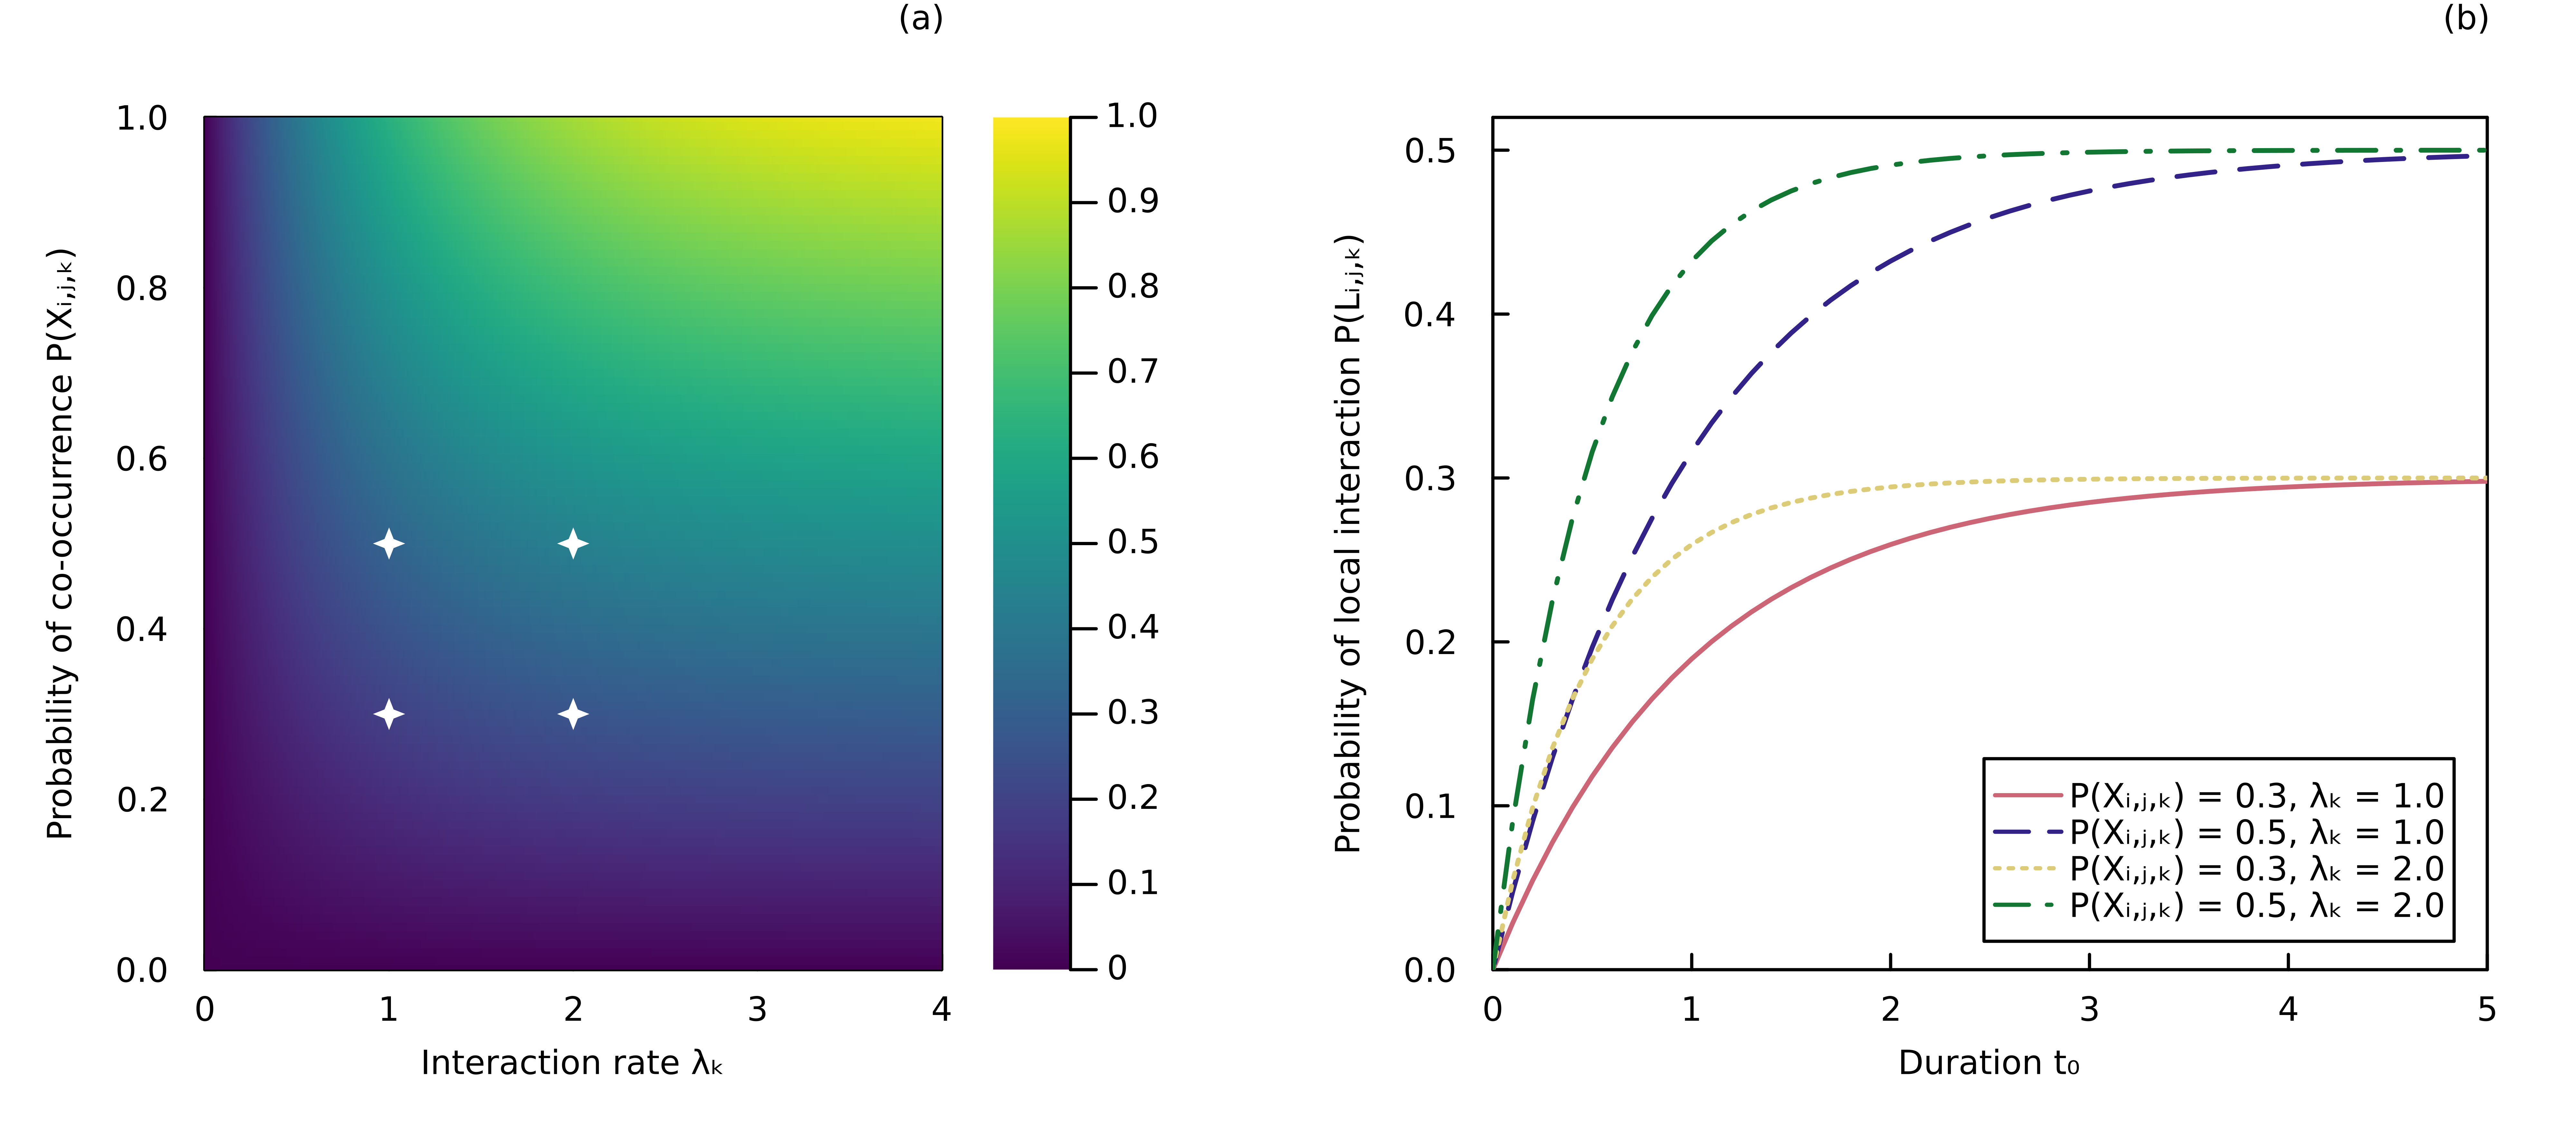
\includegraphics[width=\textwidth]{figures/article1/spatiotemporal_model.png}
  \caption{\textbf{Parameters of the spatiotemporally explicit model of interactions.}
  (a) Probability of local interaction given by the process model (Eq~\ref{eq:modeleq})
  under different values of $\lambda_k$ (interaction rate) and $P(X_{i,j,k})$
  (probability of co-occurrence), with $t_0 = 1$ (duration). The probability of
  local interaction represents the probability that the two taxa will interact
  at least once within the given time interval. Parameters $t_0$ and $\lambda_k$
  have complementary units (e.g., $t_0$ in months and $\lambda_k$ in number of
  interactions per month). The parameter values used in the right panel are
  denoted by the white stars. (b) Scaling of the probability of interaction with
  the duration parameter $t_0$, for different values of $\lambda_k$ and
  $P(X_{i,j,k})$.}
  \label{fig:spatiotemporal}
\end{figure}

\clearpage

\newtcolorbox{box1.2}{colback=green!10,enhanced,title=Box 2: Dissimilarity of local host-parasite networks,
	attach boxed title to top left={xshift=-4mm},boxrule=0pt,after skip=1cm,before skip=1cm,right skip=0cm,breakable,fonttitle=\bfseries,toprule=0pt,bottomrule=0pt,rightrule=0pt,leftrule=4pt,arc=0mm,skin=enhancedlast jigsaw,sharp corners,colframe=gree,colbacktitle=gre,boxed title style={
		frame code={ 
			\fill[gre](frame.south west)--(frame.north west)--(frame.north east)--([xshift=3mm]frame.east)--(frame.south east)--cycle;
			\draw[line width=1mm,gre]([xshift=2mm]frame.north east)--([xshift=5mm]frame.east)--([xshift=2mm]frame.south east);
			
			\draw[line width=1mm,gre]([xshift=5mm]frame.north east)--([xshift=8mm]frame.east)--([xshift=5mm]frame.south east);
			\fill[green!40](frame.south west)--+(4mm,-2mm)--+(4mm,2mm)--cycle;
		}
	}
}

\begin{box1.2}

We present a way to assess local network variability and dissimilarity
regarding species composition and interactions. We do so by comparing local
tripartite host-parasite networks to the metaweb using data from
\cite{Kopelke2017Foodweb}. This collection of networks consists of interactions
between willows, willow-galling sawflies, and their natural enemies sampled
across Europe. All data manipulation and methods are described in Appendix 1.
All code and data to reproduce these analyses are available on Zenodo
(https://doi.org/10.5281/zenodo.12802326).

In Fig~\ref{fig:accumulation}a-b, we show how the dissimilarity between the
metaweb of binary interactions and aggregated local networks changes with the
number of sampled local networks. We compared the metaweb and the aggregated
local networks using the dissimilarity in species composition ($\beta_{S}$,
Fig~\ref{fig:accumulation}a) and the dissimilarity of interactions between
common species ($\beta_{OS}$, Fig~\ref{fig:accumulation}b) indices
(\cite{Poisot2012Dissimilarity}). Expectedly, local networks are highly
dissimilar from the metaweb in terms of species composition, especially when
only a limited number of sites have been sampled. This is because few species
from the metaweb (species pool) occur locally. Moreover, we observe a peak in
the dissimilarity of interactions between common species at intermediate
sampling levels. This suggests that species are collected faster than their
interactions. With a limited number of sampled local networks, few regional
interactions are observed locally. Adding more sites brings new species, but not
always their interactions. Quadratic relationships of network properties with
sampling effort were also observed by \cite{McLeod2021Sampling}.

Next, we investigate how the number of local interactions and connectance
scale with the number of sampled (aggregated) local networks of probabilistic
or binary interactions (Fig~\ref{fig:accumulation}c-d). By comparing the scaling
relationships observed in local networks of binary and probabilistic
interactions, we observe that high values of $P(L_{i, j, k}|M_{i, j})$ lead to
systematic overestimations in the number of interactions and connectance,
especially when $P(L_{i, j, k}|M_{i, j}) = 1$ (i.e., when local and regional
probabilities of interactions are equivalent). This suggests that high values
of $P(L_{i, j, k}|M_{i, j})$ do not adequately capture the variability of
local interactions. However, these biases tend to diminish as the number of
sampled networks increases, indicating that most interactions are eventually
captured when $P(L_{i, j, k}|M_{i, j})$ is high. In contrast, low values of
$P(L_{i, j, k}|M_{i, j})$ lead to missing interactions, resulting in an
underestimation of the number of interactions and connectance. These results
underscore the importance of using the appropriate level of variability when
estimating local interaction probabilities.

\end{box1.2}

\begin{figure}[!h]
  \centering
  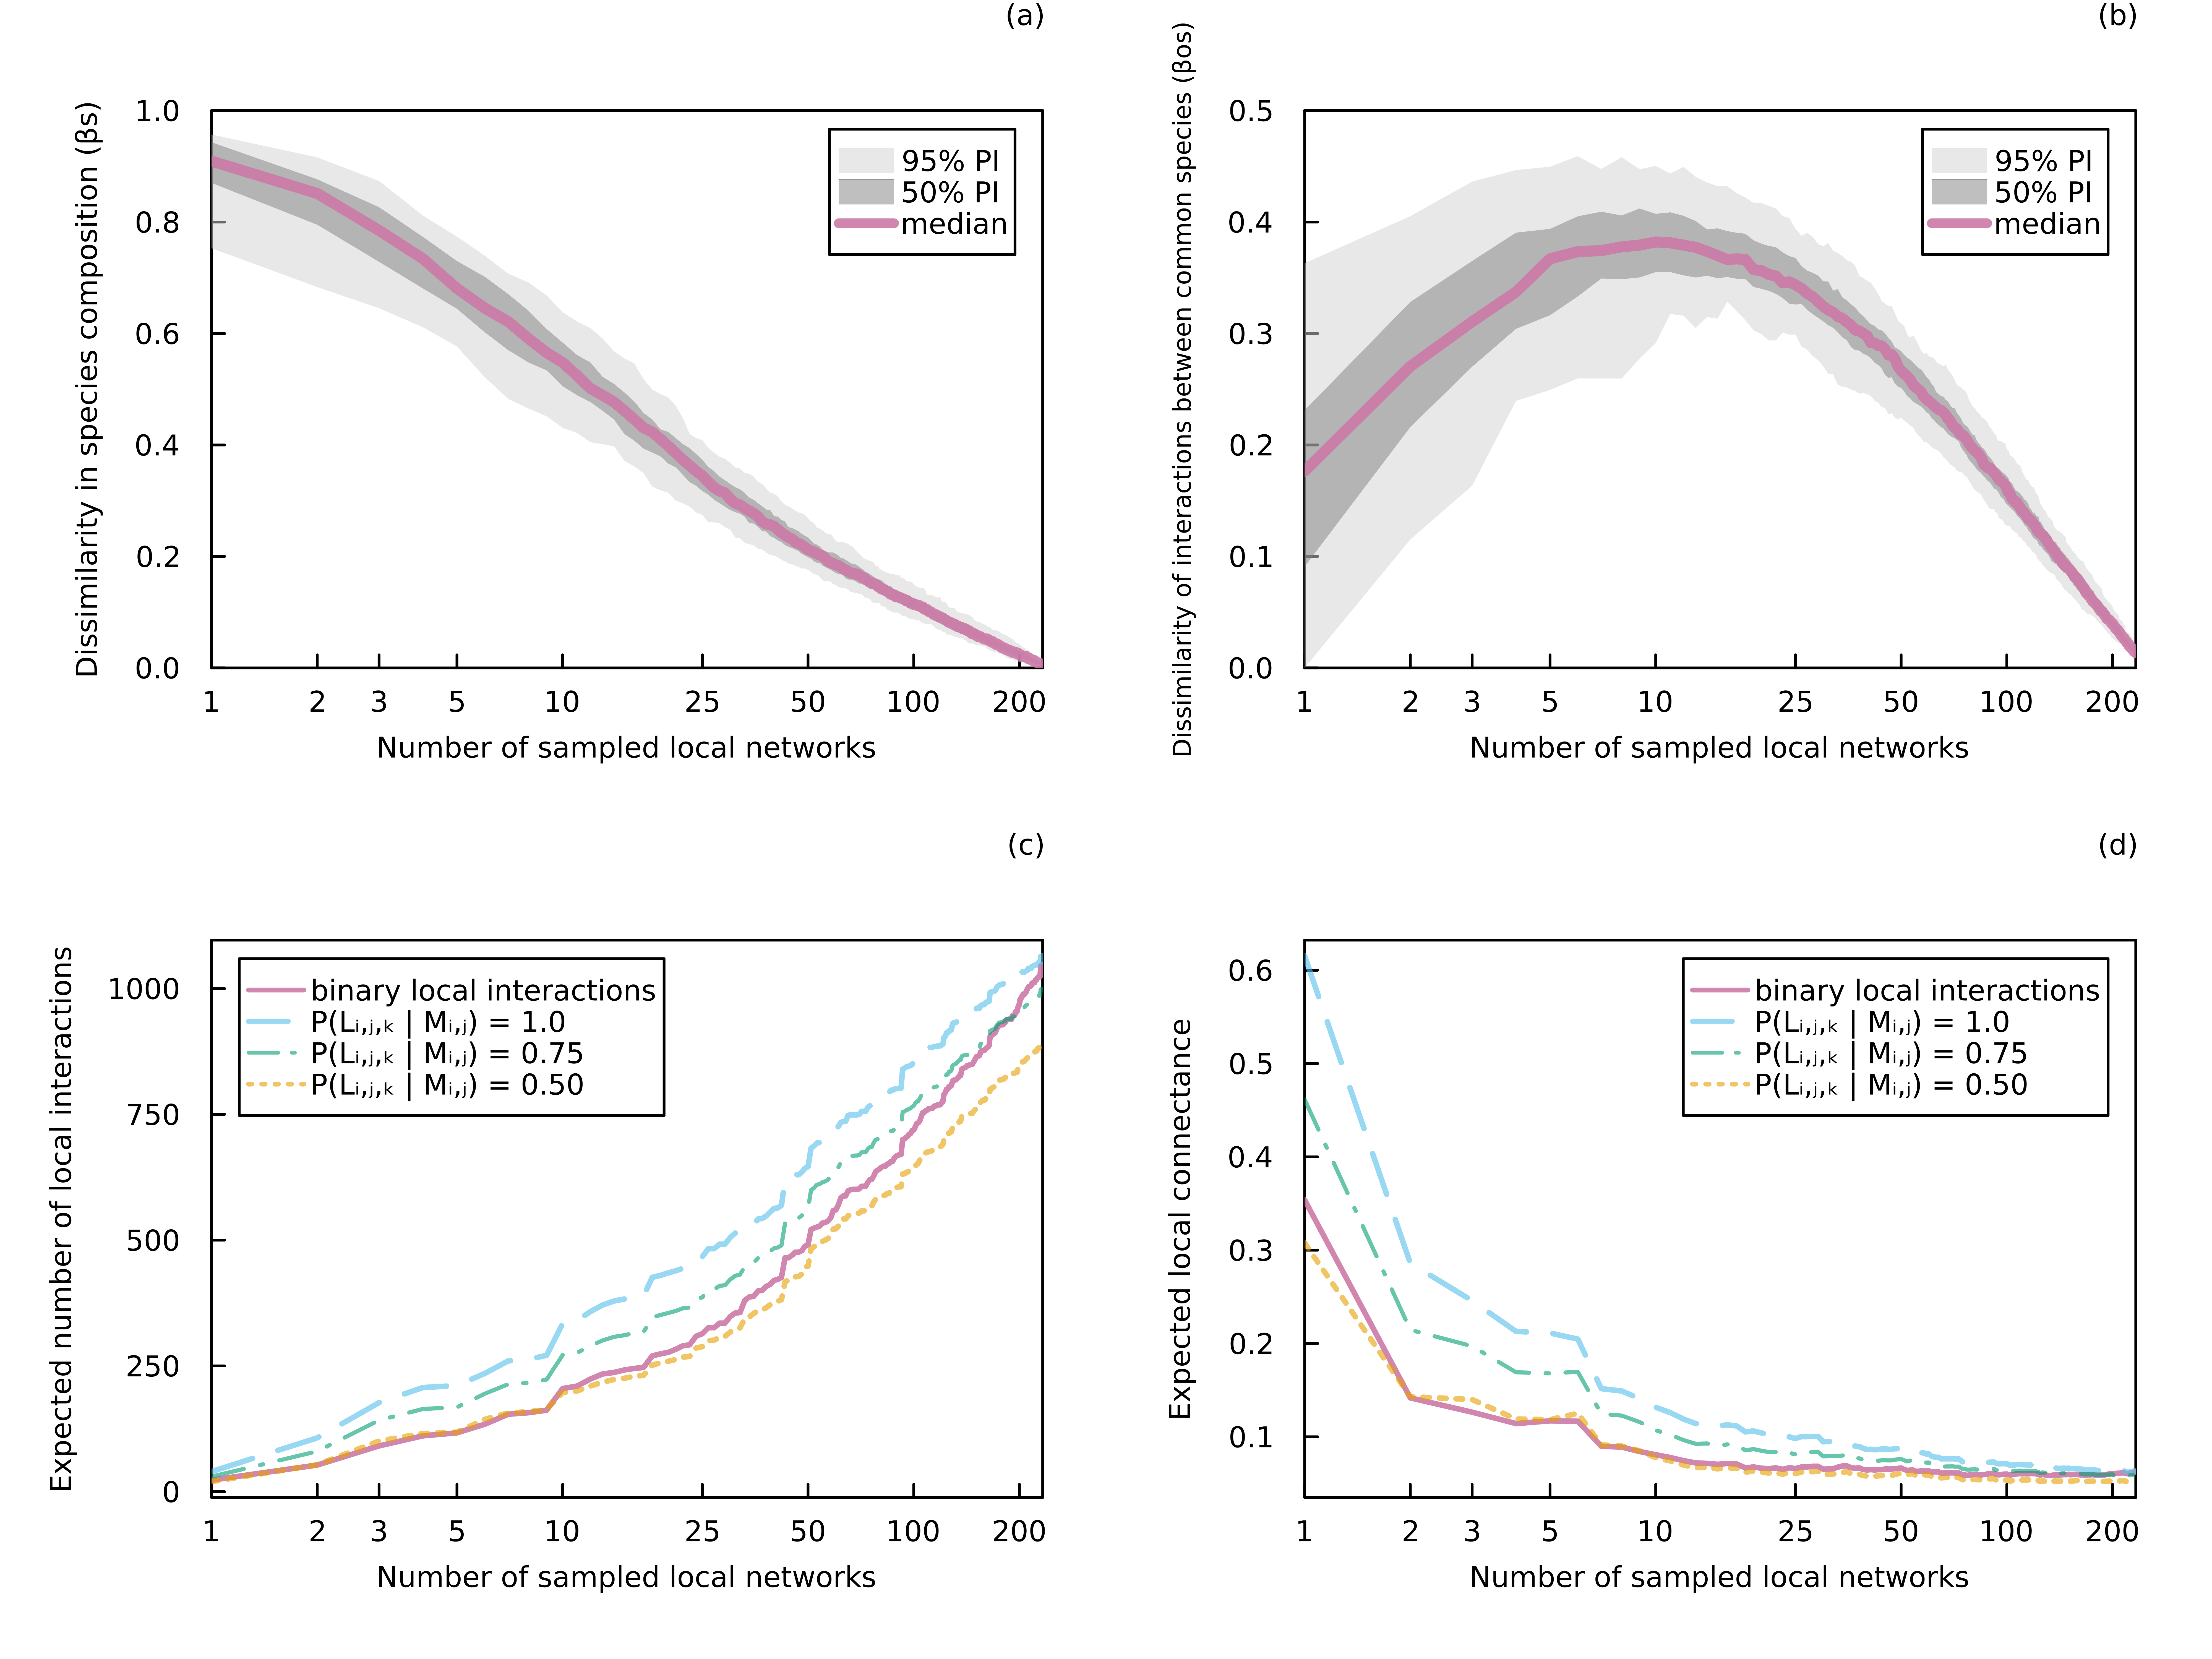
\includegraphics[width=\textwidth]{figures/article1/network_accumulation.png}
  \caption{\textbf{Network accumulation curves.}
  (a) Dissimilarity in species composition and (b) dissimilarity of interactions
  between common species between aggregated local networks and the metaweb of
  binary host-parasite interactions. In both panels, the colored line represents
  the median dissimilarity across simulations and the grey areas cover the
  $50\%$ and $95\%$ percentile intervals. (c) Scaling of the number of
  interactions and (d) scaling of connectance with the number of sampled
  (aggregated) binary and probabilistic local interaction networks. For a better
  comparison with binary interactions, local networks of probabilistic
  interactions were derived from a metaweb of probabilistic interactions with a
  false positive and false negative rate of zero. A specific value of $P(L_{i,
  j, k}|M_{i, j})$ (the local probability of interaction among potentially
  interacting species) was used for all non-aggregated local networks within a
  particular curve. Aggregated local networks were obtained by sequentially and
  randomly selecting a number of local networks and aggregating both their
  species and interactions (with the value of $P(L_{i, j, k}|M_{i, j})$
  increasing in aggregated local networks of probabilistic interactions).}
  \label{fig:accumulation}
\end{figure}

\clearpage

\section{Metawebs: regional catalogs of interactions}

\subsection{What are regional probabilistic interactions?}

Metawebs (\cite{Dunne2006Network}) are networks of potential interactions over
broad spatial, temporal, and taxonomic scales (e.g., food webs at the
continental scale). They correspond to the temporal and spatial asymptotes of
local interactions (Box 1). Potential interactions describe the biological
capacity of taxa to interact under optimal or feasible environmental conditions
given enough time, which is typically assessed at the regional scale. Metawebs
of probabilistic interactions are particularly useful in situations where there
is uncertainty in the ability of taxa to interact (\cite{Strydom2023Grapha}).
They may also be used as informative priors of local interactions. Therefore,
building a metaweb of probabilistic interactions may be an important first step
before predicting networks at finer scales. 

In contrast to local networks, where interaction probabilities arise from the
variability of interactions and the lack of information on the conditions,
interaction probabilities in metawebs solely result from a lack of knowledge.
This uncertainty arises due to insufficient interaction data, especially for
taxa that have not yet been observed to co-occur, and uncertainties in
trait-matching models. As data accumulates, interactions in metawebs should tend
towards binarity, either taking a value of $1$ (observing an interaction at
least once) or approaching $0$ (repeatedly failing to observe an interaction
between co-occurring taxa). Confidently observing an interaction once confirms
its biological feasibility, but failing to observe it (even on multiple
occasions) does not ensure that it is non-feasible (e.g., due to false
negatives, \cite{Catchen2023Missinga}). While local interaction probabilities
are irreducible because of local variability, the uncertainty of regional
interactions reduces to $0$ with the addition of information. Moreover, although
\textit{neutrally} forbidden interactions (i.e., forbidden interactions between
rare species, \cite{Canard2012Emergence}) have low probability values in local
networks, they would have a probability of $1$ in the metaweb (this is because
the species' traits could support an interaction if they were to encounter each
other at high enough abundances). Likewise, non-co-occurring taxa may have a
non-zero probability of interaction in the metaweb. Regional interaction
probabilities are thus fundamentally different from local interaction
probabilities, both in terms of uncertainty sources and probability values.

The extent of sampling effort influences our evaluation of probabilities of
regional interactions, as sampling over a larger area or for a longer duration
enables us to capture a greater number of interactions (Box 1,
\cite{McLeod2021Sampling}). However, in contrast with local networks of
probabilistic interactions, regional interactions are not evaluated for any
particular local context (they are rather a collection of local contexts), which
impacts how they scale with space and time (notably through the extent of the
region covered and sampling duration). In Box 3, we discuss the differences in
spatial and temporal scaling of regional interactions compared to local
interactions. We do so using the host-parasite networks of
\cite{Kopelke2017Foodweb} as an illustration of spatial scaling (Box 3).
Understanding the effect of spatial and temporal scales (including sampling
effort) on local and regional interaction probabilities is important for
effectively propagating uncertainty across scales and highlighting the
fundamental differences between these two types of networks. 

\subsection{What are regional probabilistic interactions conditioned on?}

\subsubsection{Regional interactions describing biological feasibility are conditioned on traits}

Potential interactions describe what we refer to as the \textit{biological}
feasibility of interactions, which is based solely on the regional traits
distributions $T_i$ and $T_j$ of taxa $i$ and $j$, respectively. We define
regional traits distributions as the range of phenotypes that a taxon can
express across various environments. Local traits $T_{i,k}$ and $T_{j,k}$, which
vary spatially and temporally because of phenotypic plasticity and local
environmental variability (\cite{Berg2010Trait}), are a subset of regional
traits. A probability of potential interaction in a metaweb $M$ describing the
biological feasibility of interactions may be expressed as: 

\begin{eqnarray}
  \label{eq:metaweb}
  P(M_{i, j} | T_i, T_j),
\end{eqnarray}

which, in contrast with local networks, is not conditioned on any spatial,
temporal, co-occurrence or environmental variables (Table~\ref{tbl:prob}).
Because phylogenetically close species often share similar traits, we should
expect that closely related species will have similar interacting partners. We
can thus use phylogeny to predict species traits and infer regional interactions
(\cite{Strydom2022Food}, \cite{Eklof2016Phylogenetic},
\cite{Stouffer2012Evolutionary}). The taxonomic level at which interactions are
evaluated also influences the distribution of regional traits. However, as
explained in Box 4, there is no fundamental difference in the taxonomic scaling
of regional and local interactions (i.e., how interaction probabilities change
with taxonomic level) because they both depend on trait aggregation. 

The biological feasibility of interactions expresses our degree of belief that
there exists at least one combination of phenotypes that could support an
interaction if they were to encounter each other, assuming they had enough time
to interact. Evaluating this probability is conducted without incorporating the
environmental conditions under which they encounter each other into the model.
It is the complement of the probability $P(F_{i, j} | T_i, T_j)$ of forbidden
interactions (i.e., the probability that their traits do not support an
interaction), which is based uniquely on biological traits:

\begin{eqnarray}
  \label{eq:forbidden}
  P(M_{i, j} | T_i, T_j) = 1 - P(F_{i, j} | T_i, T_j).
\end{eqnarray}

For example, let $i$ be a western diamondback rattlesnake (\textit{Crotalus
atrox}) and $j$, a wood lemming (\textit{Myopus schisticolor}). These two taxa
never co-occur, the rattlesnake being adapted to warm regions of North America
(\cite{Castoe2007Phylogeographic}) and the lemming, to northern habitats of
Eurasia (\cite{Fedorov2008Comparative}). As we lack direct observations of an
interaction between these two species, we have to rely on expert knowledge or
trait-matching models to estimate their probability of potential interaction. To
accurately estimate this probability using trait-matching models, it is crucial
to ensure that the set of traits considered reflects the overall traits
distributions of both taxa. We could for instance consider their average body
mass and the average phylogenetic distance of lemmings to rattlesnakes' prey.
Doing so, we might find a high probability of potential interaction based on
these traits. This example illustrates how regional interactions describing
biological feasibility may be estimated solely based on traits, without taking
into account environmental conditions (which could be important to consider when
e.g. an interaction is forbidden at all temperature values). 

\subsubsection{Regional interactions describing ecological feasibility are conditioned on traits and environmental conditions}

The biological feasibility of interactions should not be confused with what we
refer to as the \textit{ecological} feasibility of interactions. A probability
of potential interaction in a metaweb $M^*$ describing the ecological
feasibility of interactions may be expressed as: 

\begin{eqnarray}
  \label{eq:metaweb2}
  P(M^*_{i, j} | T_i, T_j, E),
\end{eqnarray}

where $E$ is the environmental conditions under which potential interactions are
evaluated (Table~\ref{tbl:prob}). Unlike $E_k$, these environmental conditions
do not represent conditions occurring at specific locations. Ecological
feasibility represents the probability that two taxa interact if they were to
encounter each other under given environmental conditions, assuming they had
enough time to interact. Incorporating environmental conditions into a
trait-matching model may be important when there is high covariance between the
environment and traits. For instance, in our example involving rattlesnakes and
lemmings, the probability of potential interaction between these two species may
be low in most environmental conditions. Western diamondback rattlesnakes may be
unactive under low temperatures (\cite{Kissner1997Rattling}), whereas wood
lemmings may have low tolerance to high temperatures
(\cite{Kausrud2008Linking}). The probability that an interaction is ecologically
feasible is always lower than the probability that it is biologically feasible,
even across all environmental conditions: 

\begin{eqnarray}
  \label{eq:feasibility}
  \int_{E}P(M^*_{i, j} | T_i, T_j, E) dE \leq P(M_{i, j} |
T_i, T_j).
\end{eqnarray}

This is because the biological feasibility of an interaction is a prerequisite
for its ecological feasibility. In other words, biological feasibility is
necessary but not sufficient for an interaction to be ecologically feasible. Our
discussion of metawebs focuses on the biological feasibility of interactions
since most methods developed for inferring probabilities of regional
interactions do not explicitly take into account environmental conditions (e.g.,
\cite{Strydom2022Food}). 

\subsection{How are regional probabilistic interactions estimated?}

Starting from a selected set of taxa, which are usually distributed within a
broad region of interest, metawebs can be built using different data sources,
including literature review (e.g., \cite{Maiorano2020Tetraeu}), aggregated
interaction data (e.g., \cite{Gravel2019Bringing},
\cite{Saravia2022Ecological}), trait-matching models (e.g.,
\cite{Shaw2024Framework}, \cite{Strydom2022Food}), and expert knowledge, which
is not a trivial challenge. Every pair of taxa that have confidently been
observed to interact at least once can be given a probability of $1$ (i.e.,
$P(M_{i, j}) = 1$) since we know that they \textit{can} interact. This differs
from local networks of probabilistic interactions, where interaction events may
remain stochastic (i.e., $P(L_{i, j, k}) < 1$) even after empirically observing
interactions due to their spatiotemporal variability. Interactions that were
never observed typically have low probability values in local networks and vary
from low to high values in metawebs, contingent upon taxa traits distributions
(reaching $0$ for forbidden links). The aggregation of model predictions and
data from different sources thus tends to raise the number of potential
interactions in metawebs.

When using local interaction data to estimate probabilities of regional
interactions, repeatedly failing to observe an interaction between two
co-occurring taxa should decrease the probability that the interaction is
biologically feasible. Using Bayes' theorem, the probability that the
interaction is biologically feasible given that it was never observed locally,
$P(M_{i, j} = 1 | O_{i, j, k} = 0)$, may be calculated as follows: 

\begin{eqnarray}
  \label{eq:emp_sampling}
  P(M_{i, j} = 1 | O_{i, j, k} = 0) = \frac{P(O_{i, j, k} = 0 |M_{i, j} = 1)
\times P(M_{i, j} = 1)}{P(O_{i, j, k} = 0)}.
\end{eqnarray}

The reduction in the probability of regional interaction after considering that
it was never observed locally (i.e., $P(M_{i, j} = 1 | O_{i, j, k} = 0) <
P(M_{i, j} = 1)$) occurs because $P(O_{i, j, k} = 0 | M_{i, j} = 1)$ must be
lower than $P(O_{i, j, k} = 0)$, i.e. there is a higher chance of observing an
interaction when it is biologically feasible. 

Observations of interactions may be false positives because of observation
errors due to taxonomic misidentifications and ecological misinterpretations,
such as those involving phylogenetically close species or cryptic species and
interactions (\cite{Pringle2020Resolving}). Likewise, forbidden interactions may
be false negatives, e.g. if they have been evaluated based on unrepresentative
or incomplete traits distributions. Employing Bayesian models proves valuable
when estimating interaction probabilities in metawebs (e.g.,
\cite{Bartomeus2016Common}, \cite{Cirtwill2019Quantitative}). This improvement
is achieved by updating prior information regarding the feasibility of
interactions (e.g., experts' prior assessments of interaction probabilities)
with empirical data on interactions and traits. By improving our estimation of
potential interaction probabilities, we may build more reliable metawebs that
adequately reflect our uncertainty on the biological feasibility of
interactions.

\newtcolorbox{box1.3}{colback=green!10,enhanced,title=Box 3: Spatial and temporal scaling of interactions,
	attach boxed title to top left={xshift=-4mm},boxrule=0pt,after skip=1cm,before skip=1cm,right skip=0cm,breakable,fonttitle=\bfseries,toprule=0pt,bottomrule=0pt,rightrule=0pt,leftrule=4pt,arc=0mm,skin=enhancedlast jigsaw,sharp corners,colframe=gree,colbacktitle=gre,boxed title style={
		frame code={ 
			\fill[gre](frame.south west)--(frame.north west)--(frame.north east)--([xshift=3mm]frame.east)--(frame.south east)--cycle;
			\draw[line width=1mm,gre]([xshift=2mm]frame.north east)--([xshift=5mm]frame.east)--([xshift=2mm]frame.south east);
			
			\draw[line width=1mm,gre]([xshift=5mm]frame.north east)--([xshift=8mm]frame.east)--([xshift=5mm]frame.south east);
			\fill[green!40](frame.south west)--+(4mm,-2mm)--+(4mm,2mm)--cycle;
		}
	}
}

\begin{box1.3}

Local networks and metawebs have distinct relationships with space (area or
volume) and time (sampling effort or duration). Local probabilities of
interaction scale both spatially and temporally, because local interactions
have more opportunities to be realized in larger areas and longer durations.
In a larger sampling area and duration, we increase the likelihood of sampling
favorable conditions for interactions to occur. If a local network of
probabilistic interactions $L_1$ with an area $A_1$ is compared to a larger
network $L_0$ with an area $A_0$, and $A_1$ is entirely nested within $A_0$,
interaction probabilities should be lower in the smaller network, i.e.
$P(L_{i,j,1} | A_1 < A_0) \le P(L_{i,j,0} | A_0)$. However, if $A_1$ and $A_0$
are disjoint, interaction probabilities could be higher in the smaller area,
contingent upon local environmental and biological conditions. In contrast,
regional probabilities of interaction do not scale with space and time. The
probability of two taxa potentially interacting should be the same in all
metawebs in which they are present regardless of scale, provided that the data
and methods used for estimation are consistent. This is because they depend
solely on the biological capacity of two taxa to interact, regardless of
co-occurrence and local environmental conditions. However, probabilities of
regional interactions may change, tending to become more definitive, with
increased sampling effort. 

In Fig~\ref{fig:spatial}, we show how the expected \textit{number} of local
host-parasite interactions scales with the spatial boundary of the network
(represented by an expanding latitudinal window) in comparison with regional
interactions. We do so using the host-parasite networks of
\cite{Kopelke2017Foodweb}. The increase in the number of regional interactions
is due to the inclusion of more species in a larger area. To ensure a
conservative comparison between aggregated local and regional networks, we
employed equal interaction probabilities (i.e., using $P(L_{i, j,k}|M_{i, j}) =
1$) in both types of network. This means that local interaction probabilities
could not increase further when aggregating them. Despite this, we notice that
the total number of regional interactions scales more rapidly than local
interactions. This is because numerous regional interactions involve species
that never co-occur, and as a result, these interactions are not captured in
local networks. All data manipulation and methods are described in Appendix 1.

\end{box1.3}

\begin{figure}[!h]
  \centering
  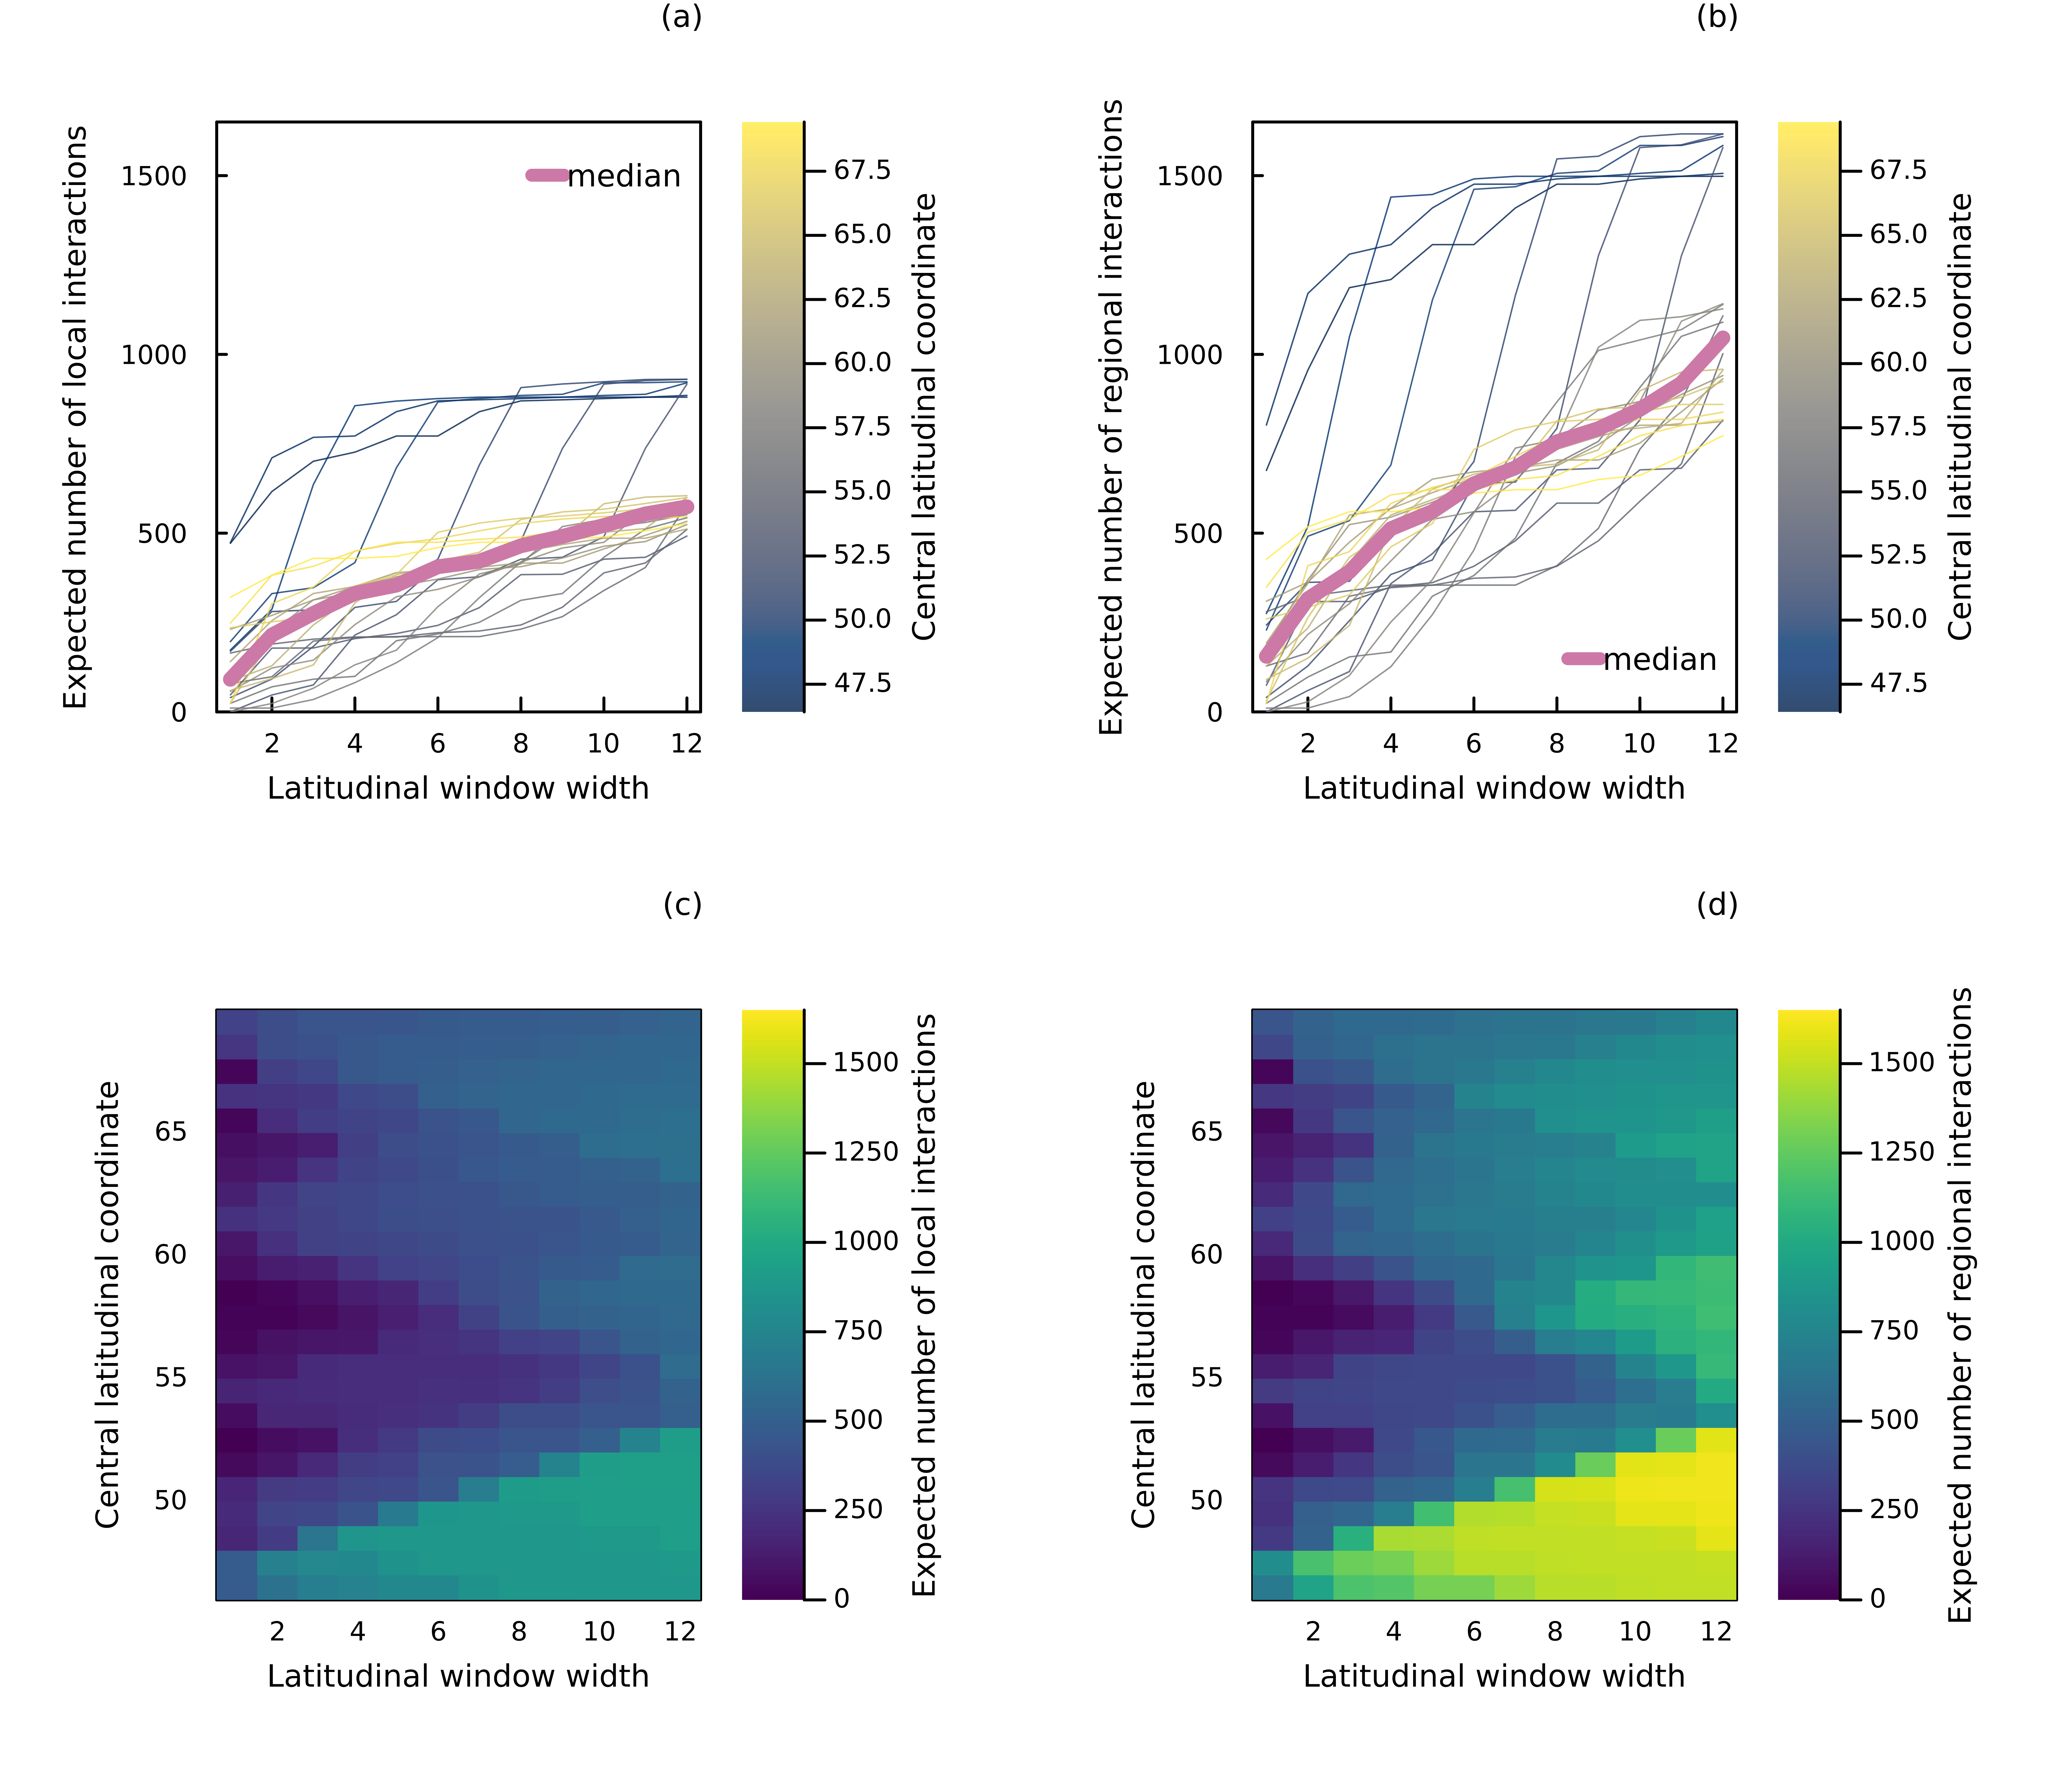
\includegraphics[width=\textwidth]{figures/article1/spatial_scaling.png}
  \caption{\textbf{Spatial scaling of interactions.}
  Expected number of host-parasite interactions in a network aggregating all (a)
  local and (b) regional probabilistic interactions within a latitudinal window
  of a given width. Every dashed curve corresponds to a different window
  centered at a given latitude (color bar), with the pink solid line
  representing the median number of interactions across windows. Heatmaps of the
  expected number of (c) local and (d) regional interactions found in windows of
  specified width and position (central latitude). Probabilities of regional
  interactions were obtained with a false positive rate of $5\%$ and a false
  negative rate of $10\%$. Local probabilistic interactions were derived from
  regional probabilistic interactions by setting the value of $P(L_{i, j,
  k}|M_{i,j})$ (the local probability of interaction among potentially
  interacting species) to $1$. Aggregated local networks were obtained by
  aggregating both the species and interactions found within a particular
  latitudinal window, with the values of $P(L_{i, j, k}|M_{i, j})$ remaining at
  their maximum value of $1$.}
  \label{fig:spatial}
\end{figure}

\clearpage

\newtcolorbox{box1.4}{colback=green!10,enhanced,title=Box 4: Taxonomic scaling of interactions,
	attach boxed title to top left={xshift=-4mm},boxrule=0pt,after skip=1cm,before skip=1cm,right skip=0cm,breakable,fonttitle=\bfseries,toprule=0pt,bottomrule=0pt,rightrule=0pt,leftrule=4pt,arc=0mm,skin=enhancedlast jigsaw,sharp corners,colframe=gree,colbacktitle=gre,boxed title style={
		frame code={ 
			\fill[gre](frame.south west)--(frame.north west)--(frame.north east)--([xshift=3mm]frame.east)--(frame.south east)--cycle;
			\draw[line width=1mm,gre]([xshift=2mm]frame.north east)--([xshift=5mm]frame.east)--([xshift=2mm]frame.south east);
			
			\draw[line width=1mm,gre]([xshift=5mm]frame.north east)--([xshift=8mm]frame.east)--([xshift=5mm]frame.south east);
			\fill[green!40](frame.south west)--+(4mm,-2mm)--+(4mm,2mm)--cycle;
		}
	}
}

\begin{box1.4}

Given that our interpretation of the properties of ecological networks depends
on their taxonomic level (\cite{Melian2011Ecoevolutionary}), investigating the
taxonomic scaling of interactions (i.e., how interaction probabilities change with
taxonomic level) is important. There are no inherent differences between the
taxonomic scaling of local and regional interactions. The taxonomic level of
interactions impacts the definition of nodes. Local and regional interaction
probabilities are not directly conditioned on taxonomic scale. However, some
conditional variables (e.g., trait distribution) may covary with taxonomic
scale. In such cases, local and regional interaction probabilities would change
taxonomically following the scaling of these variables.

In both types of interactions, transitioning to a broader level of
organization (e.g., from a species-level network $S$ to a genus-level network
$G$) can be done using interaction probabilities from finer scales. For
example, in a network with $n_1$ species of genus $g_1$ and $n_2$ species of
genus $g_2$, one can calculate the probability that at least one species from
genus $g_1$ interacts with at least one species from genus $g_2$ (i.e., the
probability that the genus-level interaction occurs) as follows:

\begin{eqnarray}
  \label{eq:taxo}
  P(G_{g_1, g_2}) = 1 - \prod_{i = 1}^{n_1}\prod_{j = 1}^{n_2}(1 -
P(S_{g_{1,i}, g_{2,j}})),
\end{eqnarray}

where $g_{1,i}$ and $g_{2,j}$ are the species of the corresponding genus and
assuming independence between species-level interactions. In contrast, a
different approach is necessary when transitioning from a broader to a finer
level of organization. This is because the knowledge of an interaction between
two genera does not guarantee that all possible pairwise species combinations
will also interact. One possible method is to build a finer-scale network by
generating probabilities of interaction through random sampling from a beta
distribution, parameterized by the broader-scale network.

Fundamentally, the taxonomic scaling of interactions involves aggregating
interactions between individuals into larger groups. Interaction probabilities
at broader taxonomic scales should thus conform to probabilities of interactions
between individuals. For example, \cite{Canard2012Emergence} built a
species-based network using simulated individual-based networks. In local
individual-based food webs, the probability that two individuals interact
reflects our degree of belief that one individual will consume the other.
Likewise, in local species-based food webs, the probability that two species
interact represents our degree of belief that \textit{at least} one individual
from the predator species will consume at least another individual from the prey
species. In that regard, taxonomic scaling is analogous to the spatial and
temporal scaling of interactions, as they all represent different ways to
aggregate individuals into broader groups (either spatially, temporally, or
taxonomically).

\end{box1.4}

\newtcolorbox{box1.5}{colback=green!10,enhanced,title=Box 5: Sampling for binary interaction networks,
	attach boxed title to top left={xshift=-4mm},boxrule=0pt,after skip=1cm,before skip=1cm,right skip=0cm,breakable,fonttitle=\bfseries,toprule=0pt,bottomrule=0pt,rightrule=0pt,leftrule=4pt,arc=0mm,skin=enhancedlast jigsaw,sharp corners,colframe=gree,colbacktitle=gre,boxed title style={
		frame code={ 
			\fill[gre](frame.south west)--(frame.north west)--(frame.north east)--([xshift=3mm]frame.east)--(frame.south east)--cycle;
			\draw[line width=1mm,gre]([xshift=2mm]frame.north east)--([xshift=5mm]frame.east)--([xshift=2mm]frame.south east);
			
			\draw[line width=1mm,gre]([xshift=5mm]frame.north east)--([xshift=8mm]frame.east)--([xshift=5mm]frame.south east);
			\fill[green!40](frame.south west)--+(4mm,-2mm)--+(4mm,2mm)--cycle;
		}
	}
}

\begin{box1.5}

Local networks of binary interactions may be predicted by performing independent
Bernoulli trials for each probabilistic interaction. This is particularly useful
when analyzing the structure of probabilistic interaction networks in the
absence of specific analytical formulas (\cite{Poisot2016Structure}), even
though it may introduce biases in our estimations when connectance is low
(\cite{Poisot2014When}, \cite{Chagnon2015Characterizing}). There are at least
two techniques to sampling binary interaction networks across space, each
predicting a binary interaction network for each location $k$ within a given
region. The first technique involves performing a single Bernoulli trial for
each pair of taxa based on their regional probability of interaction: 

\begin{eqnarray}
  \label{eq:sampling1}
  M_{i, j} \sim {\rm Bernoulli}(P(M_{i, j})).
\end{eqnarray}

In employing this technique, we predict a single metaweb of binary
interactions for each simulation. Every pair of taxa predicted to interact in
this metaweb will be treated as interacting in all localized networks where
they co-occur, i.e. $L_{i, j, k} = M_{i, j}$ when $X_{i,j,k} = 1$. This will
result in local pairwise interactions without spatial variation. 

The second technique is to independently sample each local network of
probabilistic interactions: 

\begin{eqnarray}
  \label{eq:sampling2}
  L_{i, j, k} \sim {\rm Bernoulli}(P(L_{i, j, k})).
\end{eqnarray}

This can be achieved by first generating distinct probabilistic interaction
networks for each location. Because binary interactions are sampled
independently for each location, this second technique captures network
structure across space and time more effectively. When sampling binary
interactions from local interaction probabilities, it is crucial to sample at
the same spatial scale for which probabilities were estimated to prevent
systematic biases in predictions.

In Fig~\ref{fig:sampling}, we compare the average connectance of binary
interaction networks resulting from these two sampling techniques. We sampled
regional and local interactions from our host-parasite networks of probabilistic
interactions (\cite{Kopelke2017Foodweb}), generating a number of binary
interaction network realizations for each site in the dataset. These two
sampling techniques yield different outcomes, particularly for intermediate
values of $P(L_{i, j, k}|M_{i, j})$ of $0.50$, which represent instances where
regional interactions do not consistently manifest locally (i.e., with the
largest local variability). As anticipated, we observe that sampling binary
interactions from the metaweb tends to overestimate connectance on average
compared to sampling them from local networks (Fig~\ref{fig:sampling}). We also
observe an increase in the variability of connectance when employing a single
simulation (Fig~\ref{fig:sampling}a-c, cross markers), which is a more tangible
representation of the process leading to the realization of local interactions
in nature. All data manipulation and methods are described in Appendix 1.

Both sampling techniques assume independence between interactions, which might
not hold true in reality. Covariation among interactions could exist even if we
do not explicitly condition interactions on others. For example, an interaction
between two taxa could be more probable when another interaction occurs. The
consequences of this assumption of independence on the prediction of network
structure have yet to be empirically examined. Sampling whole networks (or
graphs) instead of pairwise interactions may eliminate the need for this
assumption of independence (\cite{Battiston2020Networks}).

\end{box1.5}

\begin{figure}[!h]
  \centering
  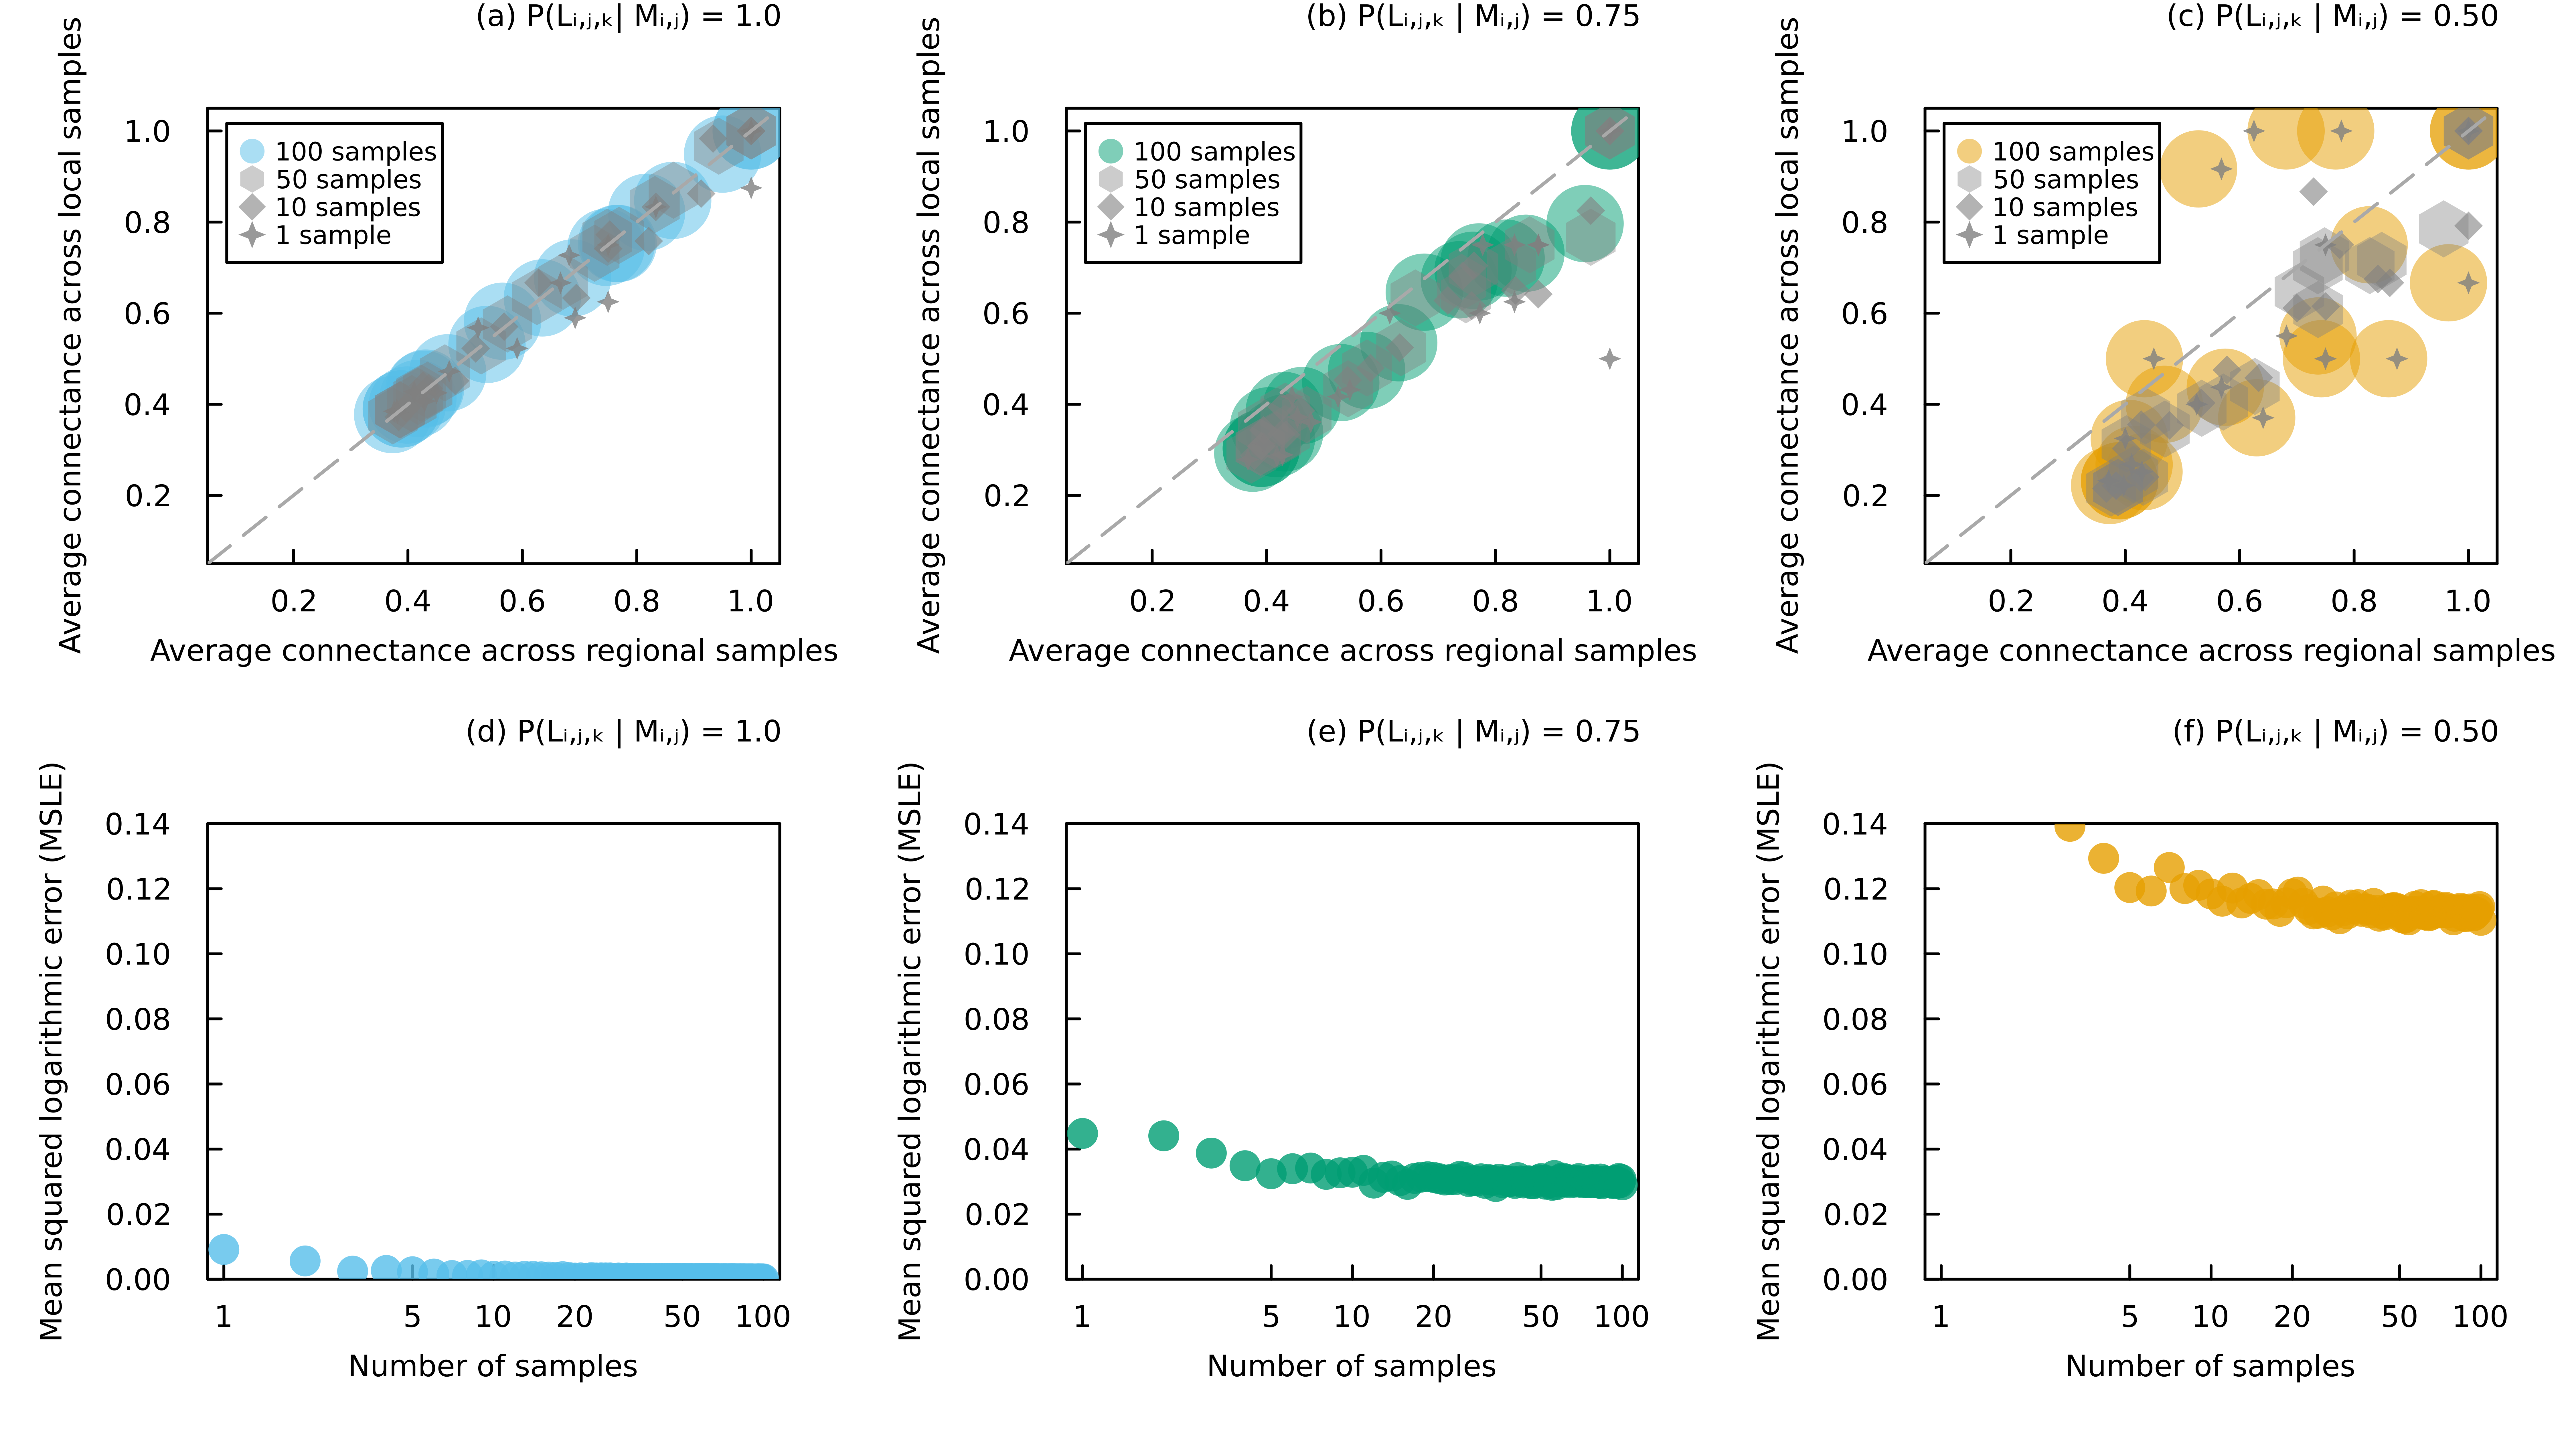
\includegraphics[width=\textwidth]{figures/article1/network_sampling.png}
  \caption{\textbf{Connectance of sampled binary interaction networks.}
  (a-c) Average connectance of binary interaction networks obtained from the two
  sampling techniques for $20$ randomly selected host-parasite networks. Cross
  markers represent the connectance of a single sample for each network, diamond
  markers the average connectance across $10$ samples, hexagon markers the
  average connectance across $50$ samples, and the colored circles the average
  connectance across $100$ samples (marker size proportional to the number of
  samples). (d-f) Reduction in the mean squared logarithmic error between the
  average connectance of binary interaction networks (all $233$ host-parasite
  networks) obtained from these two sampling techniques as the number of samples
  increases. The local probability of interaction between potentially
  interacting species was set to three different values: (a,d) $P(L_{i, j,
  k}|M_{i, j}) = 1.0$, (b,e) $P(L_{i, j, k}|M_{i, j}) = 0.75$, and (c,f)
  $P(L_{i, j, k}|M_{i, j}) = 0.50$. Probabilities of regional interactions were
  obtained with a false positive rate of $5\%$ and a false negative rate of
  $10\%$. Regional samples were obtained by randomly sampling binary
  interactions from the probabilistic interaction metaweb, and then propagating
  this result to all local networks that include the species potentially engaged
  in the interactions. Local samples were obtained by independently sampling
  binary interactions for each local network of probabilistic interactions.}
  \label{fig:sampling}
\end{figure}

\clearpage

\section{Future perspectives}

In this contribution, we underline the importance of network documentation for
adequately interpreting and manipulating probabilistic interaction data. The
mathematical representation of probabilities and their statistical properties
depend on the type of interactions (local or regional) and the conditions under
which these interactions were evaluated. We show that local networks and
metawebs of probabilistic interactions differ in their relationship to spatial
and temporal scales (Box 3), with regional interactions remaining consistent
across scales. In contrast with metawebs, local interactions are measured in a
specific context (e.g., in a given area, time, and biological and environmental
conditions) and depend on taxa co-occurrence. These differences bring to light
the need to use probabilistic data with caution, for instance when generating
network realizations of binary interactions across space (Box 5). Clear
documentation describing the type of interaction and the variables used in their
estimation are required to ensure adequate data manipulation. Sound data
practices and foundations for probabilistic thinking in network ecology
facilitate reliable assessments of the spatiotemporal variability and
uncertainty of biotic interactions. Here we identify key research priorities for
improving our understanding of probabilistic local and regional interactions.

\subsection{Predicting local networks from metawebs}

Metawebs are a valuable source of ecological information for predicting local
networks across time and space. Local networks of binary interactions can be
reconstructed by selecting a subset of taxa and interactions from the metaweb
(\cite{Dunne2006Network}). Determining the list of taxa to select can be achieved
empirically (e.g., observed occurrence data for a site) or numerically (e.g.,
species distribution models). As species composition is arguably easier to
sample and predict than pairwise interactions, the primary challenge lies in
deciding which interactions to select from the metaweb. Inferring the structure
of local networks from the metaweb before predicting local pairwise interactions
could hold promise (\cite{Strydom2021Roadmapa}), considering that the structure of
local networks is constrained by the metaweb (\cite{Saravia2022Ecological}).

While predicting local binary interactions from a metaweb is not be a simple
task, inferring local networks of probabilistic interactions from a metaweb
comes with its own set of challenges. For example, \cite{Dansereau2024Spatially}
inferred spatially-explicit food webs from a metaweb of probabilistic trophic
interactions between Canadian mammals. Their predicted localized food webs are
downscaled versions of the metaweb (i.e., localized metawebs with the same
interaction probabilities as those in the regional metaweb). To infer local
networks as defined in this manuscript (i.e., describing local realizations of
interactions), local interaction probabilities must be smaller than regional
interaction probabilities. Inferring local networks from a metaweb by
maintaining identical interaction probability values introduces systematic
biases into the predictions, as discussed in Box 2 (unless networks are seen as
downscaled metawebs).

As suggested by \cite{McLeod2021Sampling}, metawebs establish an upper limit for
local interactions (similarly for metawebs of probabilistic interactions,
\cite{Strydom2023Grapha}). In other words, the probability that two taxa interact
at a specific location and time is consistently lower or equal to the
probability of their regional interaction, regardless of the conditional
variables considered:

\begin{eqnarray}
  \label{eq:switch}
  P(L_{i, j, k} | ...) \le P(M_{i, j} | T_i, T_j).
\end{eqnarray}

Moreover, the probability that two taxa possess the biological capacity to
interact must be higher than the probability of them interacting at any location
and time because they may never co-occur or encounter locally. Specifically, the
cumulative probability of local interaction across all spatial, temporal, and
environmental conditions must be less than the probability of regional
interaction, i.e.

\begin{eqnarray}
  \label{eq:all}
  \int_{E_k}\int_{A_0}\int_{t_0} P(L_{i, j, k} | E_k, A_0, t_0) \, \text{d}t_0
\, \text{d}A_0 \,\text{d}E_k \leq P(M_{i, j} | T_i, T_j).
\end{eqnarray}

Estimating more precisely the probability $P(L_{i, j, k}|M_{i, j})$ that two
taxa interact locally if they can potentially interact allows for improved
predictions of local networks from the metaweb of probabilistic interactions.
This task is challenging due to the variability of this probability across space
and time, as well as its variability across pairwise interactions within a
network. Using simple models of $P(L_{i, j, k}|M_{i, j})$, as shown in Appendix
1, represents an initial step toward the overarching objective of reconstructing
local networks from metawebs.

\subsection{Quantifying and reducing interaction uncertainty} 

While sampling biological communities decreases the uncertainty of interactions
by accumulating evidence for their feasibility and local realization, there is a
limit to how much we can reduce uncertainty. In metawebs, probabilities reflect
our limited knowledge of interactions, which is expected to improve with a
larger volume of data. Regional interactions should become more definitive (with
probabilities approaching $0$ or $1$) as we investigate various conditions,
including different combinations of species traits. 

In comparison, local interaction probabilities represent both our knowledge
uncertainty and their spatiotemporal variability. Owing to environmental
heterogeneity, there will invariably be instances in which an interaction occurs
and others in which it does not, across different times and locations,
irrespective of the extent to which we can improve our knowledge of its
biological feasibility and the local conditions that facilitate its occurrence.
When local networks describe probabilities of observing interactions rather than
their realization, we must also consider observation uncertainty (sampling
error) as an additional source of uncertainty. Quantifying and partitioning this
uncertainty will enable us to make more accurate predictions about ecological
interactions at various spatial and temporal scales, and to identify priority
sampling locations to reduce this uncertainty. This will prove to be of vital
importance as our time to understand nature runs out, especially at locations
where the impacts of climate change and habitat loss hit harder.

\subsection{Relaxing the independence assumption} 

Estimating local interaction probabilities independently for each taxa pair and
assembling them into a network of probabilistic interactions comes with
limitations. Predicting local networks of binary interactions based on these
interaction probabilities assumes independence among interactions, a condition
seldom respected in practice (\cite{Golubski2011Modifying}). Relaxing this
assumption is the next logical step in the stochastic representation of
interactions. 

A more accurate representation of the uncertainty and variability of ecological
networks involves creating \textit{probabilistic networks} ($P(L_k)$ and $P(M)$),
rather than networks of \textit{probabilistic interactions} ($P(L_{i, j, k})$ and
$P(M_{i, j})$). Probabilistic networks describe the probability that a
particular network of binary (or quantitative) interactions (its whole adjacency
matrix) is realized. For example, \cite{Young2021Reconstruction} used a Bayesian
approach to estimate the probability of different plant-pollinator network
structures derived from imperfect observational data. A probability distribution
of ecological networks may also be derived using the principle of maximum
entropy given structural constrained (e.g., \cite{Cimini2019Statistical},
\cite{Park2004Statistical}). 

Regardless of the method used, generating probabilistic local networks could
lead to more accurate predictions of local networks of binary interactions by
bypassing the independence assumption. Probabilistic networks could serve as an
alternative to null hypothesis significance testing when comparing the structure
of a local network to some random expectations or, as done in
\cite{Pellissier2018Comparing} and Box 2, to the metaweb. These random
expectations are typically derived by performing a series of Bernoulli trials on
probabilistic interactions, assuming independence, to generate a distribution of
networks of binary interactions to calculate their structure
(\cite{Poisot2016Structure}). One could instead compare the likelihood of an
observed network to the one of the most likely network structure (according to
the probabilistic network distribution), thereby directly obtaining a measure of
discrepancy of the empirical network. Generating probabilistic ecological
networks represents a tangible challenge, one that, in the coming years,
promises to unlock doors to more advanced and adequate analyses of ecological
networks.

\section{Acknowledgment} 

We acknowledge that this study was conducted on land within the traditional
unceded territory of the Saint Lawrence Iroquoian, Anishinabewaki, Mohawk,
Huron-Wendat, and Omàmiwininiwak nations. This work was supported by the
Institute for Data Valorisation (IVADO) and the Natural Sciences and Engineering
Research Council of Canada (NSERC) Collaborative Research and Training
Experience (CREATE) program, through the Computational Biodiversity Science and
Services (BIOS²) program. A special thanks to all members of the Black Holes and
Revelations working group (organized by BIOS²) and the Poisot Lab for their
insightful discussions and valuable feedback on this manuscript.

 % Pour générer la bibliographie à la fin
 % de l'article, utiliser la commande de la
 % classe <dms> \sectionbibliography{<nom du .bib>}.
 % Il y a aussi la possibilité d'utiliser le package
 % <chapterbib>, auquel cas on utilise simplement
 % \bibliography normalement.
 %
 % IMPORTANT : Dans tous les cas, il faut faire
 %    pdflatex these
 %    bibtex chapitre1
 %    bibtex chapitre2
 %    .
 %    .
 %    .
 %    bibtex chapitreN
 %    pdflatex these
 %    pdflatex these
 %
 % où <these> est le nom du .tex principal
 % (qui contient le \documentclass).
 % bibtex a besoin du .aux de chapitre1 et
 % non du .tex. Il est parfois nécessaire
 % d'effacer le .aux et de recommencer la
 % compilation du début.
%%\bibliographystyle{amsplain} % style plain anglais ou
%% \bibliographystyle{amsplain-french} % style plain francais
%%\bibliographystyle{<style>} % autre
%% \sectionbibliography{ref.bib} %Donner le nom du .bib

\endinput
%%
%% End of file `02_article1.tex'.
